%\documentclass[12pt]{article}%
\documentclass[nofootinbib,preprint,floatfix,endfloats]{revtex4} % ,endfloats,floatfix
%\documentclass[12pt,a4paper,final]{iopart}

\usepackage[utf8]{inputenc}
\usepackage{nima,graphicx,amsmath,amssymb,color}%,hyperref}
\usepackage{mathrsfs}
%\usepackage{graphicx}
\usepackage{comment}
% \newcommand{\Ls}{\mathscr{L}}

% \newcommand{\lrto}{\leftrightarrow}
%  \marginparwidth 0pt
%  \oddsidemargin  0pt
%  \evensidemargin  0pt
%  \marginparsep 0pt
%  \topmargin   -0.25in 
% \textwidth   6.5in
%  \textheight  9.0 in
\newcommand{\RNum}[1]{\uppercase\expandafter{\romannumeral #1\relax}}
\newcommand{\outNim}[1]{}
%

\begin{document}
\title{Phases of Physical 3D Networks}
\author{Nima Dehmamy\thanks{nidami@gmail.com}, Soodabeh Milanlouei, Albert-L\'aszl\'o Barab\'asi}
\date{\today}

\begin{abstract}
Analyzing networks embedded in 3D space is crucial for understanding brain anatomy and pathologies pertaining to physical connections in the brain. 
Devising physical 3D layouts for networks is also of interest for  visualization purposes.
Additionally, given the recent advancements in 3D printing technology, 3D layouts may have practical value in design and manufacturing of complex devices. 
It is important to have efficient and economical 3D layout algorithm for networks. 
The role of network topology in layouts and the limitations it imposes on the feasibility of layouts must, thus, be studied.
We develop a minimal 3D layout algorithm for networks, inspired by force-directed layouts. 
We analyze the spatial properties of our layouts and find two phases based on link thickness and derive the phase transition criterion.  
In both phases, different network topologies turn out to be very similar in their volumetric properties and are not distinguishable based on volume. 
Relative link orientation, does differentiate the topologies when links are thin, but fails to do so at large link thickness. 
Thus, we discover a universal phase for 3D networks when link thickness is large.
We also evaluate the response of the layouts too stress. 
We find that even in terms of response to stress the different topologies behave the same in the universal phase. 
Additionally we find that the layouts behave like fluids in this phase. 
Comparing against brain literature, we find that many mammalian brains may be related to this universal phase at the level of connections between large brain regions.  
We also argue that primate brains most likely do not belong to this universal phase. 
\end{abstract}

\maketitle
%\tableofcontents

% \begin{abstract} 
% 1) Logic of problem 2) theory 3) implementation

% \end{abstract}


%\section{Introduction}
While many spatial networks \cite{barthelemy2011spatial}, such as highway systems, power grids, and subway lines, are effectively two-dimensional, 
spreading mostly close to the surface of the earth, other networks are naturally embedded inside 3D space. 
Embedding inside space will introduce a new layer of complexity and may, thereby, affect dynamical processes and other functions that the network might be involved in. In the brain, the physical connections are the foundation on which the functional network forms. 
Many diseases including Multiple Sclerosis \cite{compston2008ms,miller2007ms,miller2005ms}, Schizophrenia \cite{davis2003white,lim1999compromised,sigmundsson2001structural}, Alzheimer's \cite{mudher2002alzheimer,goedert1991tau,goedert1992tau} and Parkinson's disease \cite{bohnen2011white,beyer2006visual,hattori2012cognitive} can arise as a result of disruption of the physical network of myelinated axon fibers in the white matter. 
Due to the enormity of the number of connections among neurons, the structure of the brain needs to be economical as well \cite{bullmore2012economy,sporns2004organization,kotter2001connectional}. Developing 3D network layout models that are economical and efficient is, thus, a steppingstone in understanding the brain. 

Moreover, with the advent of cheap and accessible 3D printing technology and advancements in it, making intricate 3D devices, akin to small brains in structure, is becoming possible. 
Developing feasible 3D network models will allow us to examine 3D properties of such devices and will also be useful from a visualization perspective for networks.

%######################
Traditionally, the layout of a network is achieved from variants of the Force-Directed Layout (FDL) algorithms \cite{kamada1989algorithm,davidson1996drawing,fruchterman1991graph,barnes1986hierarchical}. 
FDL optimizes node locations so as to minimize the distance between nodes that are linked to each other, while ensuring that the network won't collapse to a point. 
This is achieved by assigning attractive, spring-like forces for linked node pairs and repulsive forces among all nodes, which decays with the distance %. Thus, nodes and links move to minimize the energy
 \cite{kabourov2015spring}.
Yet, in FDL algorithms nodes and links do not occupy volumes. Consequently, if we allot volume to the nodes and the links, crossings will occur (Fig. \ref{fig:crossings}). Such crossings are minimal for $r\approx 0$ but they increase with $r$.
%Red links are the links that have at least one crossing. 
% For a finite complex network the number of crossings eventually saturates when link thickness becomes comparable to the size of the layout.
% In FDL forces only depend on distance of nodes. 
% Thus, using FDL for a complex network leads to randomly oriented links, if the network is random enough (see supporting material (SM) section 1 for a detailed discussion).  
We can show that the number of link crossings\footnote{
The fit improves for larger number of links, of course.} grows linearly with link thickness when links are randomly oriented before it saturates (SI, sec. \ref{ap:cross}). 
Fig.\ref{fig:crossings} (C) shows this behavior in a Barabasi-Albert (BA) network.% with 100 nodes and $m=3$ minimum degree. 
%
\begin{figure}
    \centering
    %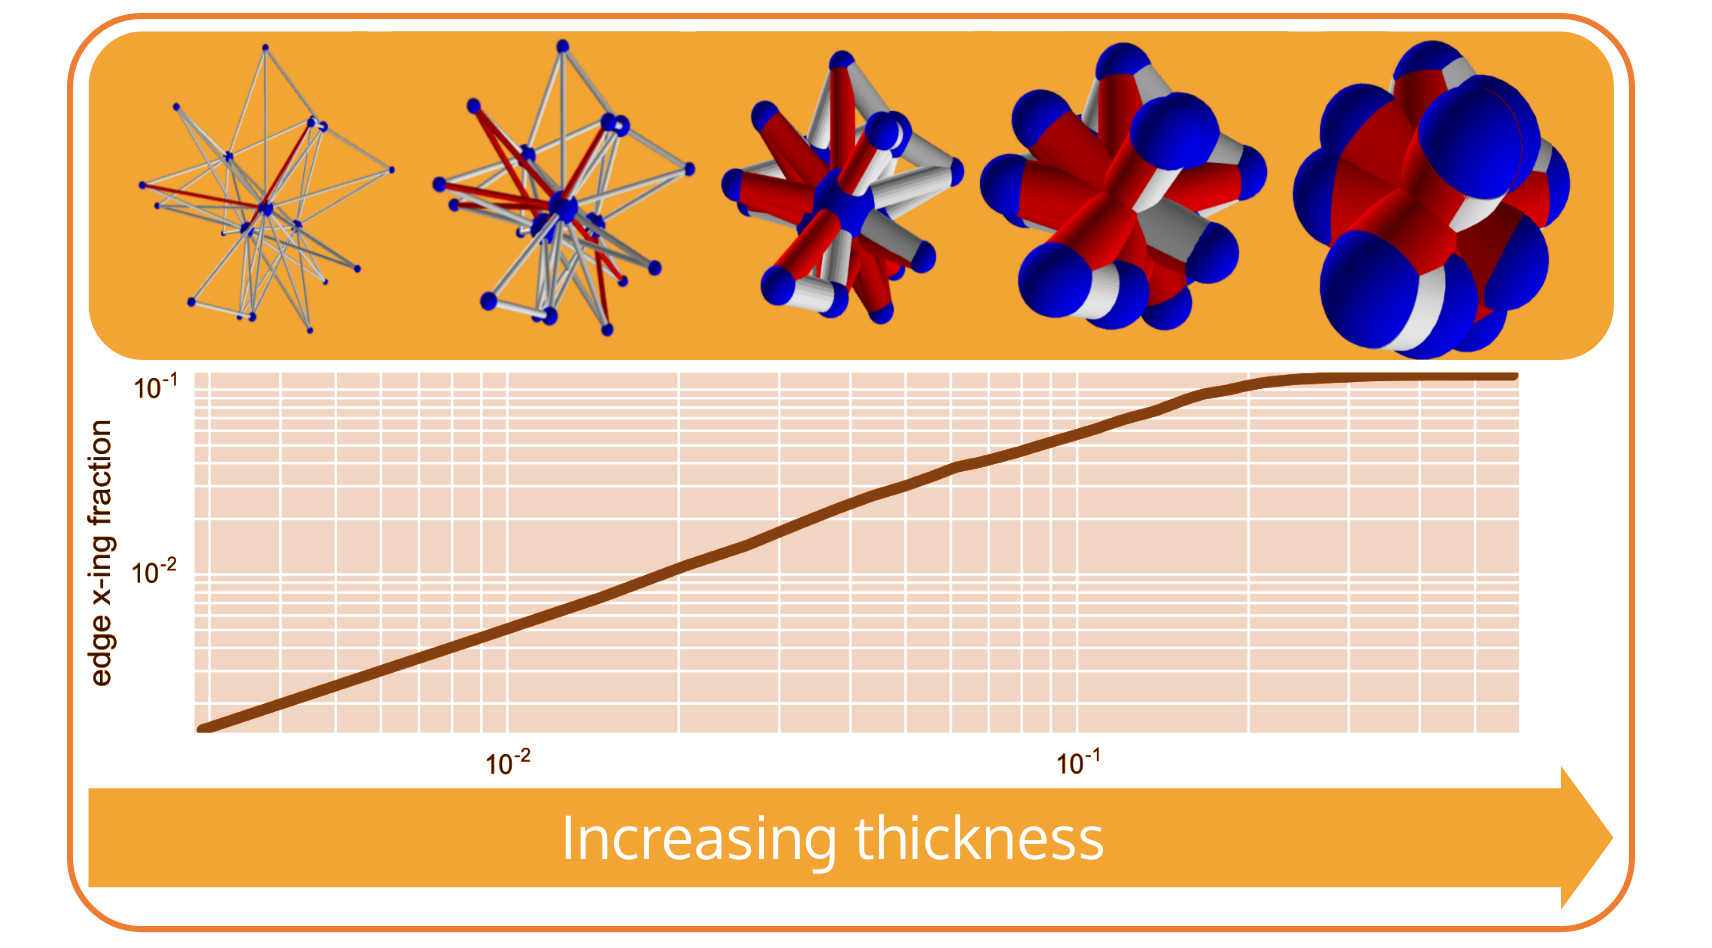
\includegraphics[width=.63\columnwidth]{fig-09-19/crs-panel.png}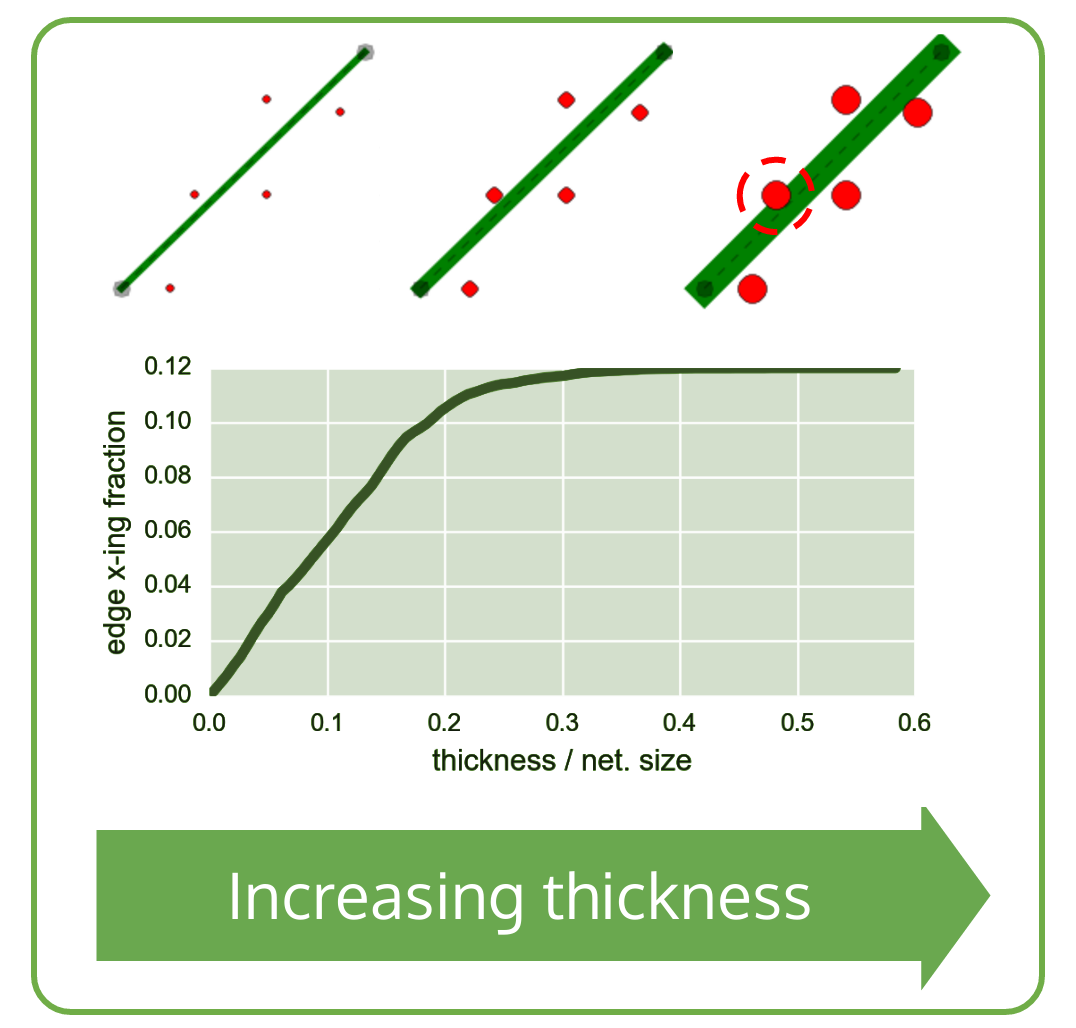
\includegraphics[width=.365\columnwidth]{fig-09-19/crs-2d-panel-green-2.png}
    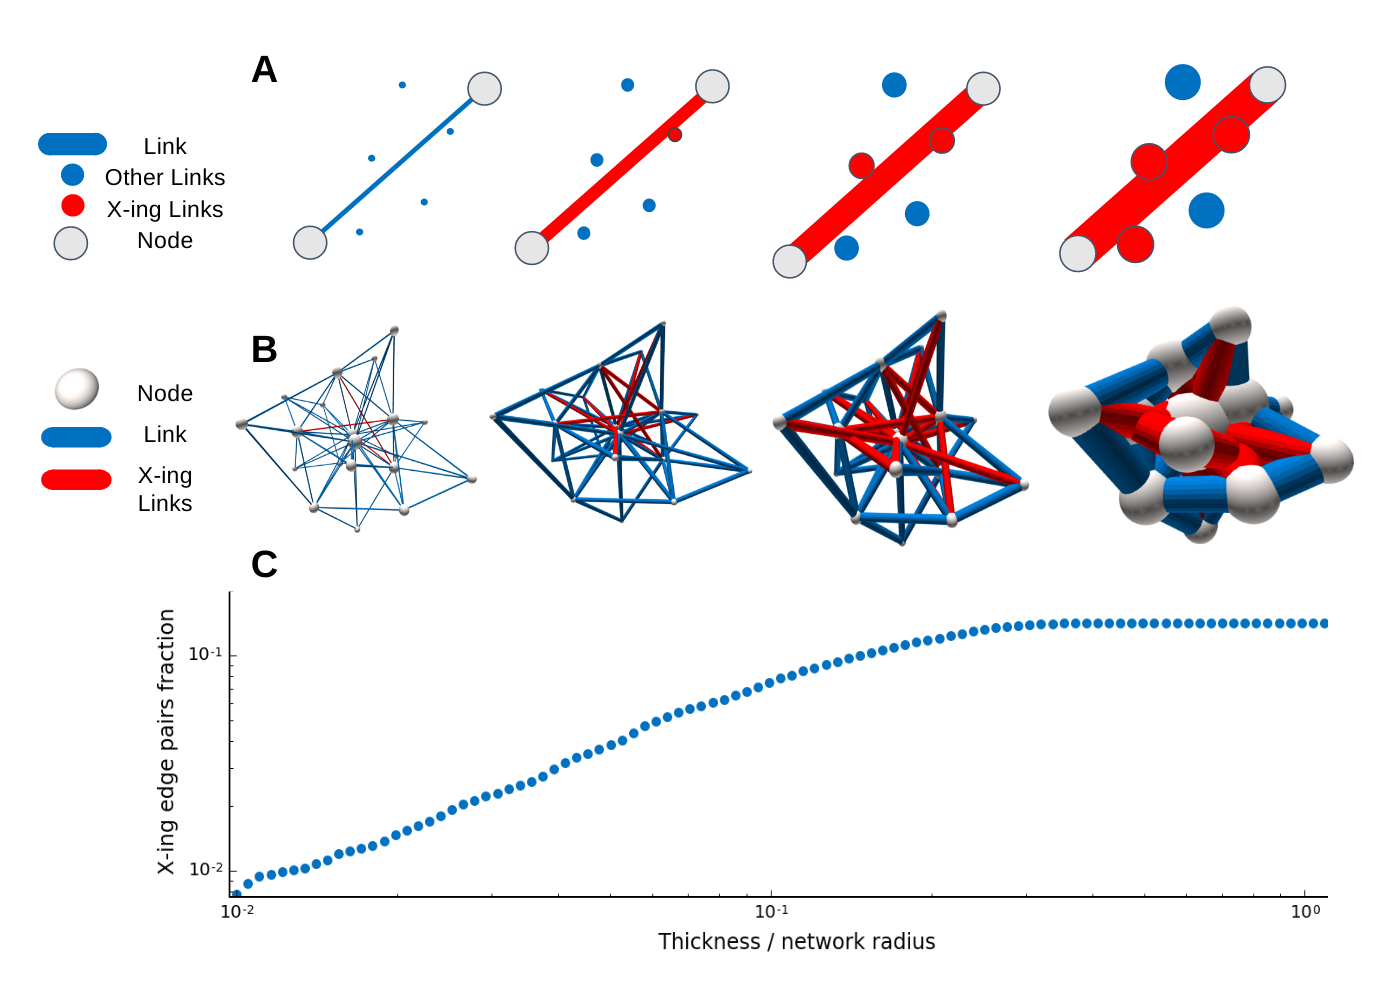
\includegraphics[width=1\columnwidth]{fig-09-19/panel-crs-2.png}
    \caption{{\bf Link crossing in FDL:} The relationship between the fraction of links crossing each other with the thickness of the links. (a) A 2D sketch of a link stretching between two nodes (light gray) and the cross section of five links going transverse to the plane. The links are blue as long as they do not touch each other. Increasing the thickness of the link, the links start crossing each other, depicted in red. (b)  Crossing links for a Barabasi-Albert (BA) network ($N = 20, m = 3$) in space, using the same color code. While increasing the thickness, the network occupies more space and crossings increase. (c) The plot shows the trend by which the number of crossings increases in a BA network with $N=100, m =3$ laid out in 3D using a popular FDL method. The number of crossings increases linearly with thickness at first, before tapering off due to finiteness of the network. It can be shown (SM) that layouts which result in random link orientations in 3D yield such linear trend in the growth of the number of crossings. }
    \label{fig:crossings}
\end{figure}

In real space-embedded networks, nodes and links have volume and links should not cross each other.
We, therefore, devise a new method to lay networks out in three-dimensional space. 
Our primary constraint in this method will be that the layout should be as economical as possible, in the sense the total volume is minimized for a fixed links thickness and node size. 
Evidently, the paths that links take must be minimized to achieve minimal volume. 
Finding the shortest path between two points is equivalent to stretching a rubber band between them (see \cite{novikov1984} and SI sec. \ref{ap:affine} for proof).
Borrowing from FDL, we model the links as rubber bands 
%As in FDL, we replace links with springs pulling their end-nodes together, 
and nodes with masses that repel each other when they are close. 
Links experience two types of force: an internal elastic force and an external repulsive force from other links.     
Forces are equal to minus the gradient of the potential energy,
which consists of an elastic potential $V_{el}= \sum_a E_a$, i.e. the sum of the elastic potential for all links $a$
(derivation in SM),
and a repulsive potential $V_{LL}$. 
To describe link-link repulsion, we introduce a Gaussian repulsive potential (SM). 
The total potential energy of the links is
\begin{align}
    V &= V_{el} + V_{LL} \cr 
    &= {k\over 2}\int dl_a {d\vec{x}_a\over dl_a} \cdot {d\vec{x}_a\over dl_a} + 
    \sum_{a\ne b} \int \int dl_adl_b 
    A \exp\left[- {|\vec{x}_a-\vec{x}_b|^2 \over 4 r_0^2}\right] \label{eq:Vfull}
\end{align}
where the integrals are over the paths that links $a$ and $b$ take. $l_a$ is the variable parametrizing the length of link $a$ and  $\vec{x}_a(l_a,t)$ represents the position of a point along the core of the link at a point at a given value of the parameter $l_a$.  
%Note that the positions on the links $\vec{x}_a(l_a,t)$ are functions of both time and the length parameter $l_a$, which means that each component is a two parameter field.  
%The equations of motion will just have one extra force term, other than the familiar gradient of $V$. This other term measures stress and tension in along the links. 

To produce the desired layout we must find the optimal configuration of nodes and links under the influence of the forces by dynamically evolving the system till it reaches minimum potential. 
We model the dynamics as a dissipative process, thereby allowing the system to converge towards a stationary state. 
To do so, we assume the space to be a high viscosity medium, introducing strong friction to the system.
Strong friction makes the equations of motion first order gradient descent instead of second order Newton's equations.
The full equation of motion for links is, thus, given by 
\begin{align}
    \eta {dx_a \over dt} & =  -{\ro V \over \ro x_a} + {d\over dl} {\ro V \over \ro (dx_a /dl)}   \label{eq:Langevin0}
\end{align}
where for clarity we have removed the position indices. Here $x_a$ is one component of $\vec{x}_a(l_a,t)$. 

%######The links are of course attached to nodes at their endpoints and the dynamics of nodes will be coupled to that of the links.

In the first iteration of our model, which we call the ``Elastic Link Model'' (ELM), we fix the position of nodes using FDL and let links reorganize themselves. 
%Later, we relax this condition and allow nodes to moves as well. 
The equilibrium layout is found by %configuration of the network we must evolve 
running the dynamics using  \eqref{eq:Langevin0} until the force terms on the right hand side of \eqref{eq:Langevin0} become vanishingly small\footnote{The choice of how small they should be is arbitrary, but it must be such that $dt$ times the right hand side is much smaller than the link thickness or node repulsion range.}. 
%Solving equations \eqref{eq:Langevin0} yields an equilibrium configuration in which
In the end, all links have shrunk to a size where the elastic and the repulsive forces on every infinitesimal link segment cancel out. 
Fig. \ref{fig:resolve} describes how ELM works and shows  simulations done using ELM. 
Fig.\ref{fig:resolve} (A) ``Theory'' sketches the idea and Fig.\ref{fig:resolve} (A) ``Simulation'' shows a simulation where ELM has resolved the crossing of three links (red links). 
The picture on the left and right refer to before and after applying ELM, respectively. In Fig. \ref{fig:crossings} (B) a 2D cross-section of a link similar to  Fig. \ref{fig:crossings} (A) is shown.
This time the link is evolved using ELM and it bends and curves to avoid crossing the links transverse to the plane (blue circles). 
%
\begin{figure}
    \centering
    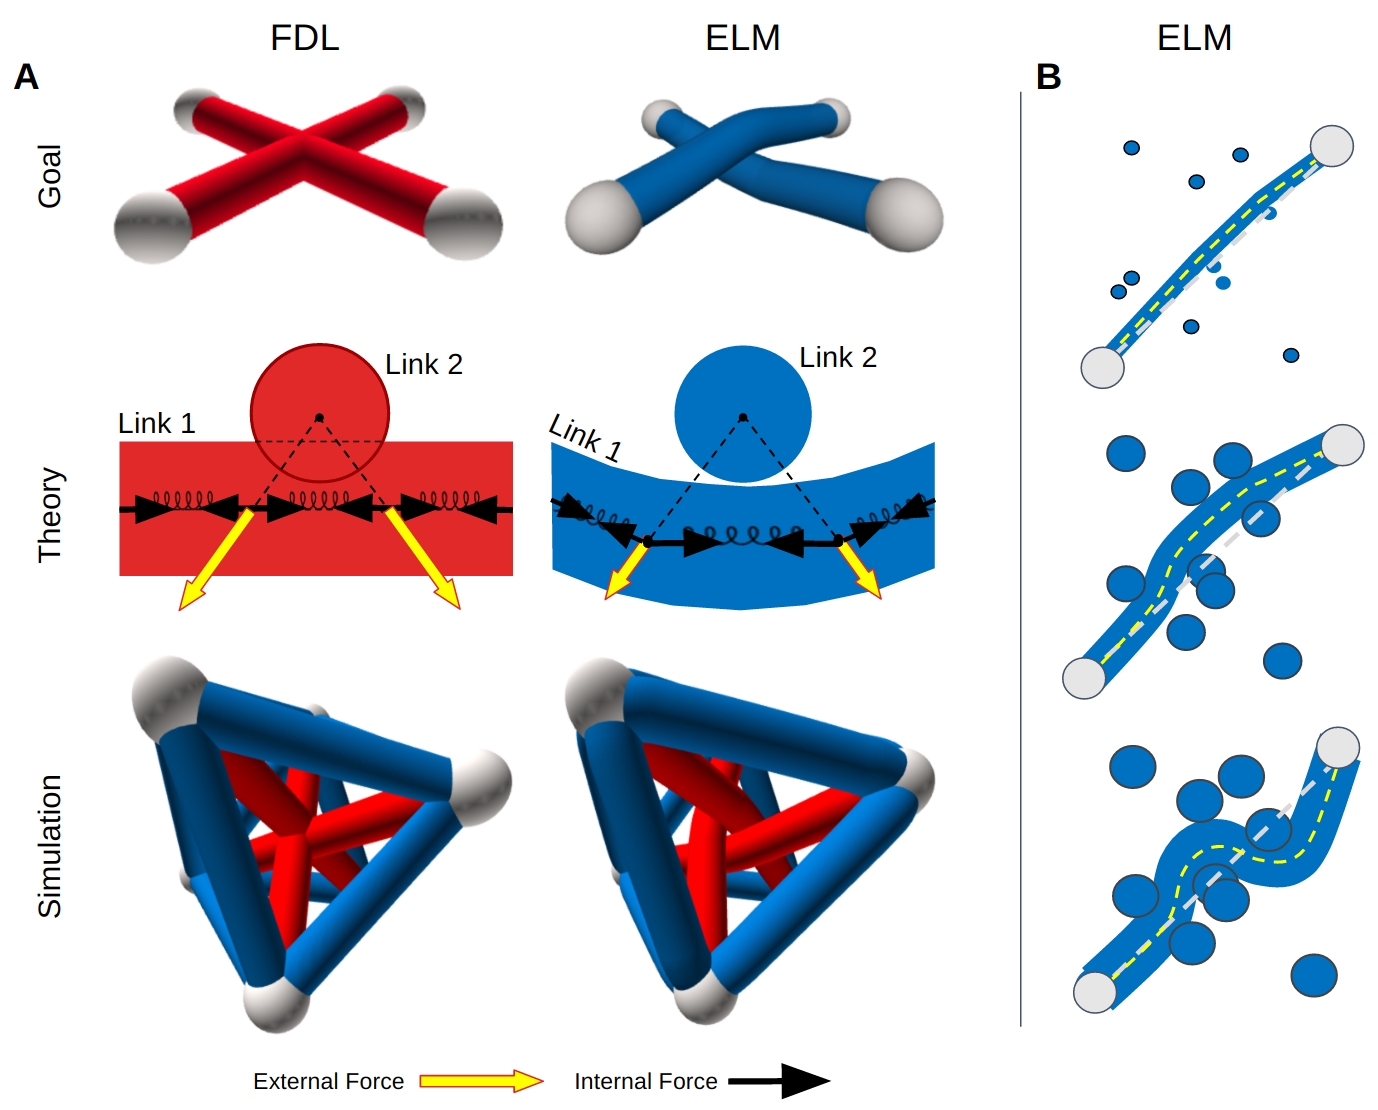
\includegraphics[width = .8\columnwidth]{fig-09-19/elf-resolve-2d.png}%{fig-09-19/force-resolve-6.png}
    \caption{{\bf How ELM works:} We simulate the elastic links as a stretched, flexible rubber band, which can be thought of as many short springs connected to each other. The elastic forces, $\mathrm{F}_{\mathrm{in}}$ of these springs is shown by the orange arrows. Links exert a repulsive force $\mathrm{F}_{\mathrm{ext}}$  on each other that falls sharply at radii larger than the link thickness $r_0$. 
    A) First and second plot sketch how the ELM resolves crossing (red) links. The bottom panel shows a complete graph with 6 nodes. Image on the left is laid out with FDL. The three red links all cross at the center. The right plot shows how the graph after simulating ELM on it, after which the red links no longer cross. B) ELM in 2D for gradually increasing link thicknesses. The blue dots are fixed obstacles whose radius is the same as the thickness of the link. Note that in the plot on the bottom the link has chosen a suboptimal path. This is  expected in these systems where the global optimum is hard to find. Other runs of the same initial conditions find other paths, thanks to the noise from simulated annealing. To obtain better results we can choose the best out of several runs.}
    \label{fig:resolve}
\end{figure}
%
The upper half of Fig. \ref{fig:ELM} shows the ELM layout for a small Barabasi-Albert (BA) network with $N=10, m=3$ at four different thicknesses. At very small thicknesses link crossing is rare and the layouts are essentially the same as the initial FDL. At very large thicknesses, however, there is no room for links inside the region where the nodes are. The links, thus, get pushed outward and make long arcs from outside to connect their endpoints.

ELM has a natural size restriction due to fixed node positions (Fig. \ref{fig:crossings}).
Consider the minimal ``bounding sphere'', i.e. smallest sphere that encloses all nodes. 
The diameter of the bounding sphere is of the order of the network size $L$. 
In a random network with $N_l$ links, using FDL results in links that have lengths comparable to $L$.\footnote{The more structured and ordered the graph is, the shorter will be the average link length. 
For instance, FDL on a regular lattice network results in a lattice layout in which links are not as long as $L$.} 
The most compact way to fit links inside a volume (see SI, sec. \ref{ap:cross}) is to stack them in parallel, a case in which the total cross section of links, $\pi r^2 N_l$, will be of order of the layout cross-section $\pi L^2/4$. 
Thus at link thicknesses $r_\mathrm{max} \sim L/O(N_l^{-1/2})$ links will make arcs outside of the bounding sphere %Beyond a certain link thickness, links will not fit inside this sphere. Gradually increasing the thickness  results in layouts that have more and more of links that make long arcs going outside of the bounding sphere 
Fig. \ref{fig:ELM}. Note that this issue happens at thicknesses much smaller than $r/L = O(1)$ where the plateau starts (Fig. \ref{fig:crossings}).  

% \section{Emancipating the ELM}
To avoid the size limit of ELM and to get more realistic layouts for large link thicknesses,
%when link thickness times average degree becomes comparable to node radius 
%(e.g. from volume available to each node based on volume of convex hull of network) 
%When the volume occupied by the links becomes comparable to the size of the layout avoiding crossing becomes impossible. 
%Now, under more relaxed and realistic circumstances, 
we allow the nodes to be free as well. 
We do so by assuming that the nodes exert a repulsive force on each other.  
In FDL, the repulsive force between nodes is generally a long-ranged electrostatic force, falling as $F \propto r^{-2}$. 
However, such long-range forces rarely exist in biological systems\footnote{Even in polymers, interactions are often modeled with the Lennard-Jones potential \cite{lennard1924determination}, which falls as $r^{-6}$ at large distances and like a hard-core interaction in very short distances. }.
%We do not want the nodes to have only a hard-core interaction with each other, but also that they maintain a distance from one another. 
Also, in the interest of understanding spatial properties, having a short-range %repulsive 
force that falls sharply beyond a certain distance %between nodes 
would give us more control over the network size. Therefore, we choose to model the repulsive force among nodes based on a Gaussian potential. %, which gives us more control over the distances between interacting nodes than a $r^{-2}$ force does. 
%The fact that the Gaussian-force has a short range also makes it more appealing for comparison to biological systems. %{\color{red} Check behavior of long-range forces!} 
This way, the equation of motion for the node positions is given by
\begin{equation}
    \lambda_N {d\vec{X}_i\over dt} = - \vec{\del}_{\vec{X}_i} \left[V_{\mathrm{end}} + \sum_j V_{ij} \right]. \label{eq:nodes}
\end{equation}
where the node-link potential $V_{\mathrm{end}}$ and the total node-node interaction potential $V_{NN}$ are given by 
\begin{align}
    V_{NN}&= \sum_{i\ne j} V_{ij} = \sum_{i\ne j} %|d\vec{x}_a| |d\vec{x}_b|
A_N \exp\left[- {|\vec{X}_i-\vec{X}_j|^2 \over r_N^2}\right]\label{eq:VIJ}\\
 V_{\mathrm{end}} & =\left. k\sum_{i=1}^N \vec{X}_i \cdot \sum_{a\in <i>}  {\vec{x}_a%\pr{l^{(\mathrm{end})}_a}
 \over dl_a}\right|_{l_a = l^{(\mathrm{end})}_a}
\end{align}
where $r_N$ denotes the range of the repulsive node-node interaction. 
$<i>$ signifies the set of links connected to node $i$, and $l_a^\mathrm{(end)}$ being the link length parameter value at the endpoints of link $a$.
% Nodes will also be pulled by the links they are connected to. 
Together with \eqref{eq:Langevin0}, these equation constitute an extended model, which we call the Emancipated ELM (E-ELM). 
The E-ELM layout for BA network with $N=10, m=3$ at four different thicknesses is shown in  
Fig. \ref{fig:ELM}, bottom. The situation at very small thicknesses is similar to ELM (Fig. \ref{fig:ELM}, top). ELM and E-ELM start diverging at large thicknesses. E-ELM does not exhibit the long arcs observed in ELM. In E-ELM the large thickness layouts look like scaled versions of each other. Overall, the E-ELM layouts are much less dramatic than ELM and retain a reasonable shape at even very large thicknesses.
%
\begin{figure}
    \centering
    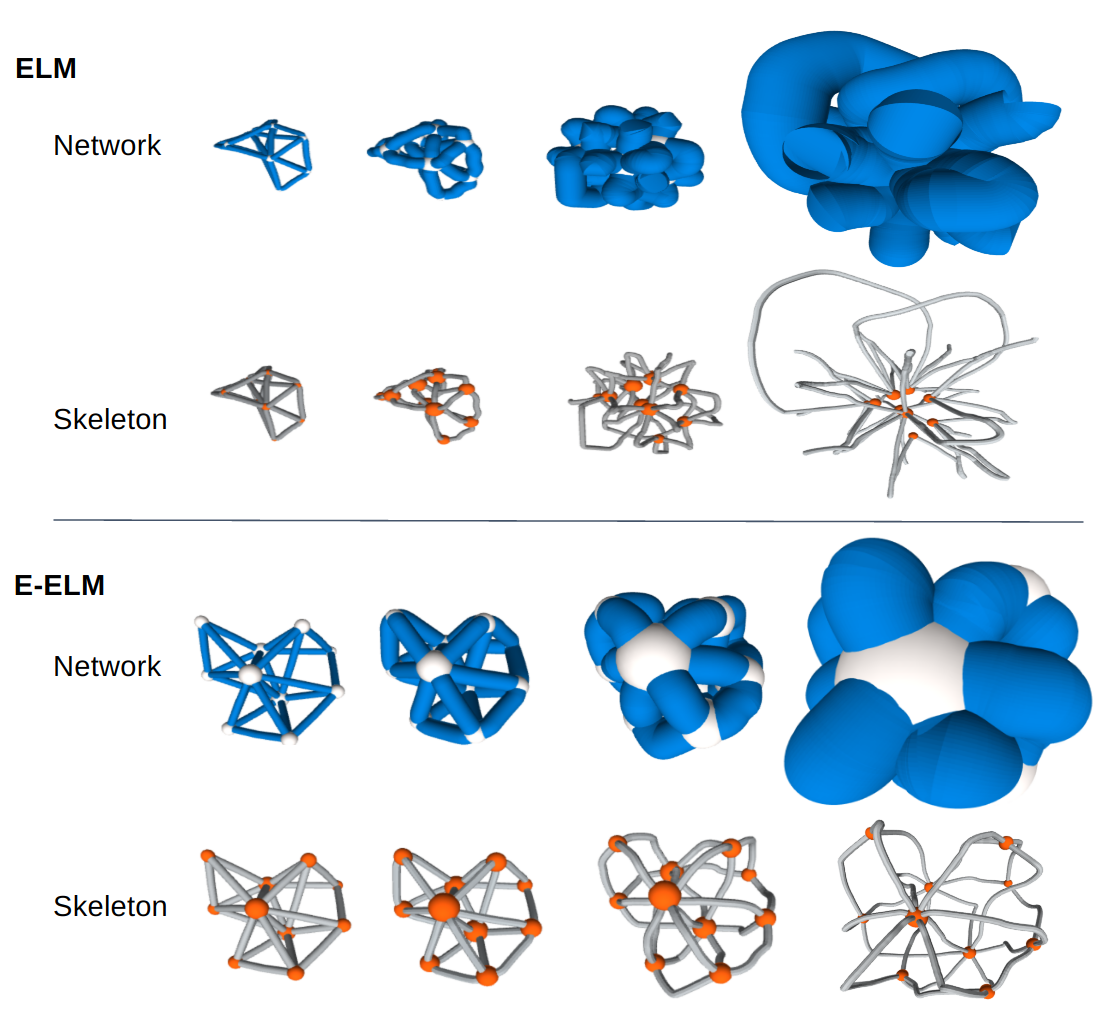
\includegraphics[width = .7\columnwidth]{fig-09-19/ELM-E-ELM.png}
    \caption{{\bf ELM and E-ELM at various link thicknesses:} ELM and E-ELM used on a BA $N=10, m=3$. Pictures with blue links are actual size. Gray links are thinned down to show the skeleton of the layout.  At small thicknesses, $r$, both layouts are the similar to FDL. At larger $r$ in ELM links start bending to avoid each other. At very large $r$, links don't fit inside the region containing the nodes and start making outward arcs. E-ELM at large $r$ behaves more gently and the layout size just grows linearly with the $r$.}
    \label{fig:ELM}
\end{figure}
%As for the transition point, 

E-ELM does not have the same space limitations as ELM, so we expect the behavior of the layout to be different at different thicknesses. 
For instance, when the link thickness is much smaller than node repulsion range ($r\ll r_N$) the size of layout $L$ is essentially determined by $r_N$ and the number of nodes $N$ through
$ L^3 \sim Nr_N^3 $. % \quad \Rightarrow \quad R \sim N^{1/3} r_N$
When links are thick ($r = O(r_N)$) %for $N_l$ links of thickness $r_l$ we have 
the layout will be comprised of closely packed links and the cross sectional area of the layout, $\pi L^2$, is comparable to the cross section of all links ($ N_l r^2 \sim L^2$). % (for $N_l$ links of thickness $r_l$).%, so $R \sim N_l^{1/2} r$. 
Therefore the transition in the behavior should happen where the two estimates for $L$ become comparable, that is when 
\begin{equation}
    {r\over r_N} \sim N^{1/3} N_l^{-1/2}. \label{eq:trans}
\end{equation}

\outNim{
\begin{figure}
    \centering
    \includegraphics[width = .7\columnwidth]{fig-09-19/{E-ELM}.png}
    \caption{{\bf ELM at various link thicknesses:} ELM used on a BA $N=10, m=3$. At small thicknesses $r$ the layout is the same as FDL, while at larger $r$ links start bending to avoid each other. At very large $r$, links don't fit inside the region containing the nodes and start making outward arcs.}
    \label{fig:E-ELM}
\end{figure}
} %%%%%%%%
%
\outNim{
\begin{figure}
    \centering
    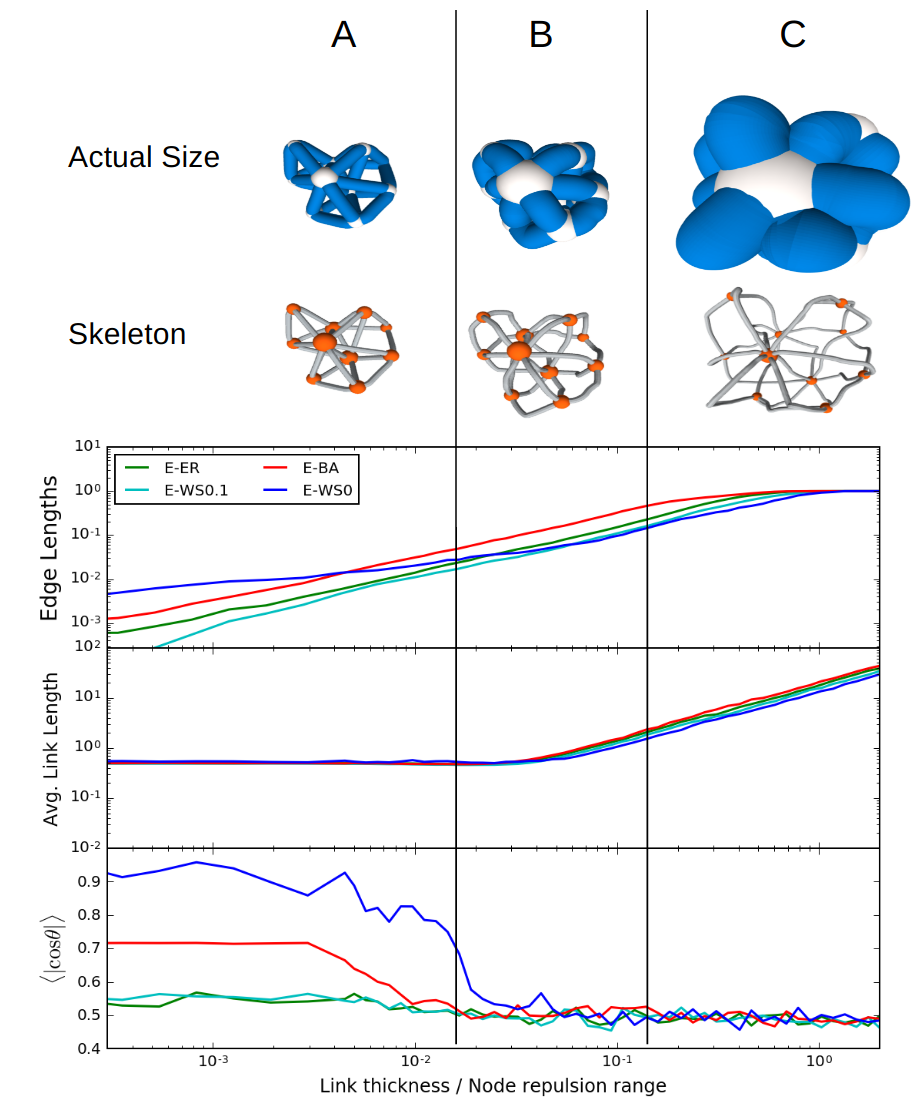
\includegraphics[width=.6\columnwidth]{fig-09-19/phase-eman-5.png}
    \caption{1}
    \label{fig:phase-eman}
\end{figure}
} %%% 

\outNim{
\begin{figure}
    \centering
    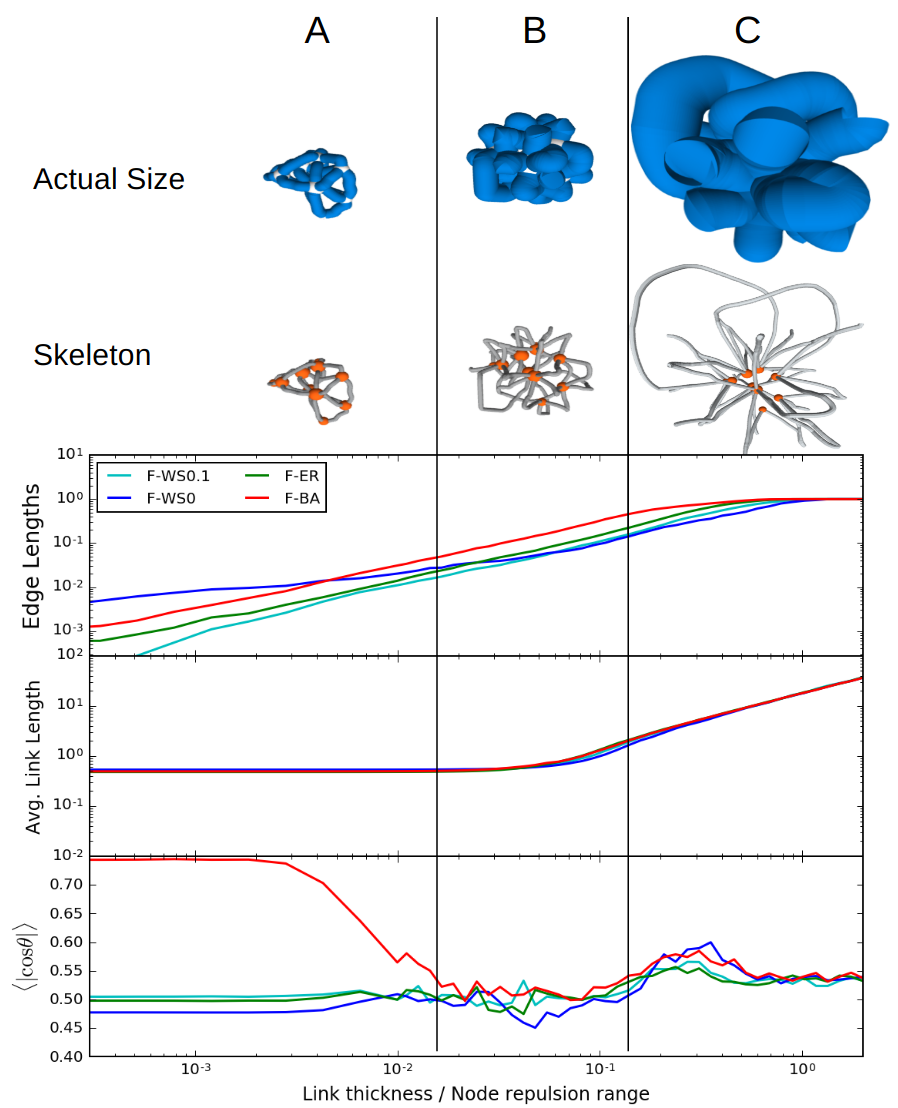
\includegraphics[width=.6\columnwidth]{fig-09-19/phase-fixed-2.png}
    \caption{{\bf Phases of the ELM:}  Top: Actual size examples of ELM and their skeletons (where links are made thinner to see their paths) for a small BA network. 
    Bottom: Dependence of two order parameters, the average link length $\be{l}$ and relative adjacent link orientations $\be{|\cos\theta|}$, ...on shows the average of cosine of angles between neighboring link segments. 
    We observe a striking rise in $\be{\cos\theta}$ after the transition which suggests that neighboring segments become more parallel. }
    \label{fig:ELMphases}
\end{figure}
}%%%

%\subsection{Locla Minima}
It is known, from studies of polymers and spin-glasses, that a complex system of interacting links has a very uneven potential energy ``landscape'' \cite{parisi2002physical} with a multitude of local minima\footnote{In the space of all possible configurations of the paths the links take.
If we approximate links as a collection discrete segments, this space will be finite dimensional, with dimensions equal to the number of segments. 
For truly smooth links, this space is the space of all smooth paths and is ill-defined mathematically, for the same reason that path integrals are ill-defined.}.
In fact, 
the equations obtained from \eqref{eq:Langevin0} are almost identical to field equations describing polymer dynamics and are a special case of general manifold dynamics \cite{mezard1991replica}. 
Hence finding the globally optimal configuration is virtually impossible. 
Since the elastic potential energy in ELM is a measure of the total length of links, local minima in the potential correspond to cases where links are following paths in which total link lengths is not minimized. 
Rather, the configuration is optimal relative to small fluctuations in the paths. 
Finding the global minimum in such systems is generally an NP hard problem.
We, therefore, use simulated annealing \cite{hwang1988simulated} to escape from highly undesirable local minima and reach an energetically more favorable local minimum. 
To do so, we perturb the paths of the links by adding thermal noise, which enables them to occasionally pass through other links and potentially find a shorter path between their end-nodes.
If the noise level is sufficient to allow tunneling through energetically costly configurations, it will result in a much more desirable layout.
We use an exponential cooling schedule to reduce the thermal noise and allow the system to converge to an equilibrium state. 

%\textit
% \section{Characterizing the layouts}

In both ELM and E-ELM layouts, a qualitative structural difference is evident at small $r$ compared to large $r$ (Fig. \ref{fig:ELM}). Despite the fact that at small $r$, ELM and E-ELM look very similar, the outcome at large thicknesses looks distinctive. 
We characterize this qualitative change in the layout within both ELM and E-ELM. In particular, we examine whether spatial characteristics of layouts differ among various network topologies which can direct us to quantify the disparity between ELM and E-ELM. 

% Looking into Fig. \ref{fig:ELM} top and bottom, there is a qualitative difference in the structure of the ELM layouts at small $r$ compared to large $r$, which is also true for E-ELM.
% However, despite the fact that at small $r$ ELM and E-ELM look very similar, the outcome at large thicknesses looks very different. 
% We characterize this qualitative change in the layout within ELM, and within E-ELM. 
% In particular, we want to see whether spatial characteristics of layouts differ  among various network topologies. We also wish to quantify how ELM and E-ELM differ. 

To explore the spatial  %organizational and volumetric 
properties of the layouts, we define functions that describe the state of a given layout, so-called ``order parameters''. 
We examine the dependence of order parameters on dimensionless parameters to make a comparison between different networks. 
Aside from the number of nodes and links, % wiring diagram, 
one dimensionless parameter is the ratio of link thickness to the (appropriately defined) size parameter of the initial layout\footnote{
In our model the spring constant $k$ and the amplitudes of repulsive forces $A$ and $A_N$ are dimensionful and determine the time-scale of the dynamics.
Also, the repulsive force can be chosen differently. }. 


% To explore the spatial  %organizational and volumetric 
% properties of the layouts, we define functions that characterize the state of a given layout, so-called ``order parameters''. 
% In order to compare different networks, we examine the dependence of order parameters on dimensionless parameters.  
% Aside from the number of nodes and links, % wiring diagram, 
% the only dimensionless parameter is the ratio of link thickness to the (appropriately defined) size parameter of the initial layout\footnote{
% In our model the spring constant $k$ and the amplitudes of repulsive forces $A$ and $A_N$ are dimensionful and determine the time-scale of the dynamics.
% Also, the repulsive force can be chosen differently. }. 


As for the choice of order parameters, the average length of links -- determining the volume of the layout -- is one natural choice.  
We rescale the initial layout of the simulations in order to make them the same size, so that a direct comparison of average edge lengths makes sense. To define the dimensionless parameter, we divide link thickness by a size parameter. 
In ELM and E-ELM, the size parameter is the diameter of the bounding sphere and the node repulsion range respectively. We choose the scale of ELM and E-ELM layouts such that at very thin links the diameter of the layouts match. 


% As for the choice of order parameters, the average length of links -- determining the volume of the layout -- is one natural choice.  
% We will rescale the initial layout of all simulations in order to make them the same size, so that a direct comparison of average edge lengths makes sense. To define the dimensionless parameter, we divide link thickness by a size parameter. 
% In ELM the size parameter is the diameter of the bounding sphere and in E-ELM, it is the node repulsion range. 
% In order to compare ELM and E-ELM, we will choose the scale of ELM and E-ELM layouts such that at very thin links the diameter of the layouts match. 

%\section{Simulation Results}
%We now use ELM to understand how networks behave at different link thicknesses. We also want to know whether different network topologies exhibit different properties in their layouts. 
We explore the behavior of various network topologies laid out using the ELM and E-ELM algorithms. 
To compare different network topologies, we fix the number of nodes and links. 
%We show simulations with $N=49$ nodes and $N_l\approx 280$ links. 
We analyze a range of network architectures, from an Erdős-Renyi (ER) random graph, to slightly more structured Barabasi-Albert (BA), 
to the highly regular 3D regular lattice (Lat).
%to 2D Watts-Strogatz (WS) with different rewiring probabilities (WS0.1: 2D with rewiring probability $p=0.1$; WS0: without rewiring). 
Fig. \ref{fig:phase-compare} shows the average link length $\be{l}$ and average adjacent link segment orientation $\be{|\cos\theta|}$ at different link thicknesses $r$. 
For both ELM and E-ELM we can divide the behavior of the order parameters roughly into two phases: a ``weak exclusion phase'' at low $r$, where links have little interaction, and a ``strong exclusion phase'', where link exclusion is the dominant interaction. The pink vertical strip signifies the transition point predicted in \eqref{eq:trans} 
\[{r\over r_N} \sim N^{1/3} N_l^{-1/2}\approx 0.22\]
that is the point near which we expect the phase transition to occur. 
For both ELM and E-ELM our estimate works very well\footnote{A more accurate analysis can be done by looking at the derivative of the order parameters (see SM) which confirms the transition point.}. 
Regarding the behavior of $\be{l}$ at various $r$, curiously, all network topologies show comparable link lengths and the same trend for different $r$ (Fig. \ref{fig:phase-compare}).
We cannot clearly discriminate between different topologies using $\be{l}$. 
It also does not distinguish ELM from E-ELM. 
At least with the assumption of the layout seeking to minimize link lengths, our finding suggests that all networks may have similar phase diagrams for average link length. 
%There are differences in the details of the transition between ELM and E-ELM, which become clear while examining $ d\be{l}/dr$ (see SM), but the contrast is not sufficient to categorize different networks. 
In the weak exclusion phase, link crossing is rare and layouts resemble FDL.
$\be{l}$ changes minimally in both ELM and E-ELM\footnote{
In SI we show that in the weak exclusion phase of ELM links do grow slowly with the number of crossings because of the fixed nodes and the dents created in the links when avoiding crossing. 
In E-ELM, however, this change is almost absent because the nodes can rearrange and allow links to become straight again.}. 
In the strong exclusion phase, all topologies show a linear trend of growth $\be{l} \propto r$, for both ELM and E-ELM.
This suggests that layouts at different $r$'s may merely represent the scaled versions of the same layout.
For ELM, %the way this should be understood is that 
in the strong exclusion phase the links are significantly thick that very few of them fit inside the bounding sphere of nodes. 
Increasing $r$, the bounding sphere effectively becomes a point at the origin and all layouts are essentially made up of links with both endpoints being the origins. 
%\footnote{While this does not seem realistic, in cases such as myelinated axons in the white matter the axon makes up only a fraction of the core of the fiber and  the full thickness of the fiber is less important to the network. }  
In E-ELM the reason the layouts become similar is that in the strong exclusion phase $r > r_N$ and, therefore, links push against each other to the extent that the distance between nodes becomes larger than their repulsion range $r_N$. This means that $r_N$ will no longer play a role in determining the size of the network. The only significant length scale is $r$ and the layout size scales linearly with $r$. 

For all network topologies and for both ELM and E-ELM, the $\be{l}$ curves coincide, 
when adjusted for number of nodes and links. This leads us to the following conclusion: 
If a class of 3D networks is laid out in space by solely minimizing link length, the phase diagram of $\be{l}$ should only consist of the two phases we observed in Fig. \ref{fig:phase-compare}. 
%Conversely, if $\be{l}$ curves looks different for a class of networks, its layout cannot have been based only on minimizing link length.

%So far, we have seen that the dependence of link length $\be{l}$ on $r$ cannot discriminate between different network topologies, or between ELM and E-ELM. 
$\be{l}$ does serve as a reasonable order parameter to distinguish the weak exclusion and the strong exclusion phase. 
%Aside from the average length of the links, t
To examine whether network topologies can be distinguished from each other in each of the weak and strong exclusion phases, we examine two other order parameters. 
One is another mathematical invariant, beside $\be{l}$,  that can be constructed from link paths, %a set of paths in Euclidean space 
which is their relative orientation. 
This information is encoded in the relative angle between link segments that touch each other. To measure it, we  first find the tangent vectors to the paths of two adjacent links at the point they touch.  Then we calculate the cosine of the angle between these two  vectors. 
Since the link-link repulsion is short-range, 
%Since the interaction of links with each other is a short-range repulsion, %we examine cosine of the angle $\cos\theta$ of link segments that touch each other. 
%we measure %analyze two different order parameters constructed from $\cos\theta$. One  is 
we will examine $\langle |\cos\theta |\rangle$, where the average is over all adjacent link segments of different links. The third order parameter is the young modulus of elasticity of the layout, which will be discussed later. 

Applying FDL to random networks,  %such as Erdős-Renyi, 
%yields a completely random set of link orientations. 
the distribution of $|\cos\theta |$ turns out to be a uniform distribution between 0 and 1, with a mean $\langle |\cos\theta |\rangle \approx 0.5$ (see SI sec. \ref{ap:cross}). 
A value $\langle |\cos\theta |\rangle > 0.5 $, thus, indicates that adjacent link segments tend to go more parallel to each other than random. 
Conversely, if they become more perpendicular we should find $\langle |\cos\theta |\rangle < 0.5 $. 
$\be{|\cos\theta|}$, on the other hand, helps us discriminate between different network topologies (Fig. \ref{fig:phase-compare}). 
Calculating $\be{|\cos\theta|}$, we only consider segments where links touch each other. 
The value of $\be{|\cos\theta|}$ doesn't change much at small $r$, despite the fact that the number of crossings is steadily growing with $r$ (Fig. \ref{fig:phase-compare}).
Interestingly, ELM and E-ELM  generally result in different values of $\be{|\cos\theta|}$ in the weak exclusion phase. 
ELM on the 3D lattice, which is not a random network, has no crossings at low $r$ and the average $\be{|\cos\theta|}$ (which only counts edges touching each other) is near zero in the weak exclusion. But in the strong exclusion phase when the links start touching, the lattice also approaches ER and BA on the $\be{|\cos\theta|}$ curve. 
%WS0, which is not a random network and has a lattice-like structure, shows the very high value $\be{|\cos\theta|} \sim 0.9 $ in E-ELM, suggesting that segments touching each other became more parallel. 
%In contrast, ELM yields  $\be{|\cos\theta|} \sim 0.5 $ for WS0, which is the same as randomly oriented segments. For other topologies, in the weak exclusion phase, $\be{|\cos\theta|} $ does distinguish between topologies, but yields more or less the same values in both ELM and E-ELM. In E-ELM, the more structured and ordered the topology, the higher seems to be the level of parallelism.  
Applying the E-ELM on the 3D lattice yields a somewhat different result. Since we used short-range node repulsion in E-ELM, the lattice's long-range order is not respected and it become a little distorted. This results in a few links touching each other, yielding a non-vanishing $\be{|\cos\theta|}$.

% Something interesting also happens in the strong exclusion phase. 
However, in the strong exclusion phase of E-ELM, all topologies become indistinguishable and $\be{|\cos\theta|} \sim 0.5 $, indicating the loss of the organization and parallelism that appeared in the weak exclusion phase. 
In the E-ELM strong exclusion phase, links touching each other neither go parallel nor perpendicular to each other.
Rather, they may go in any direction randomly\footnote{Merely  $\be{|\cos\theta|} \sim 0.5 $ doesn't prove this. But looking at the distribution of $|\cos\theta|$ we do observe that it becomes an almost uniform distribution between 0 and 1, thereby confirming the random orientation.}. 
Consequently in E-ELM, %network topologies 
in the strong exclusion phase %cannot be distinguished 
neither average link length, nor relative orientations sets different network topologies apart\footnote{
There are small differences in the slope of $\be{l}$ and the exact point where the phase transition occurs, as is to be expected.
However, these differences don't seem large enough to characterize the topologies.}. 
There is only one, universal, strong exclusion phase in terms of both $\be{l}$ and $\be{|\cos\theta|}$. 
%Whether other order parameters could discriminate between various topologies remains to be investigated. 

ELM in the strong exclusion phase exhibits a richer structure. 
First note that even using $\be{|\cos\theta|} $, topologies cannot be distinguished in the the strong exclusion phase. 
Increasing $r$ first leads to a rise in $\be{|\cos\theta|} $ up to about $0.6$, which indicates higher parallelism. 
$\be{|\cos\theta|}$, then, decreases again, eventually stopping to change with $r$, reaching a final value of $\be{|\cos\theta|} \approx 0.55 $, indicating the emergence of a degree of parallelism. 
However, this is not surprising, given the fact that at large $r$ all links point radially outward for most of their paths. Thus, links going next to each other will have a large value of  $\be{|\cos\theta|}$. The precise value of $\be{|\cos\theta|}$ at large $r$ then depends on the number of links, as having more links means the angle of adjacent links will be smaller when they go radially. 

\begin{figure}
    \centering
    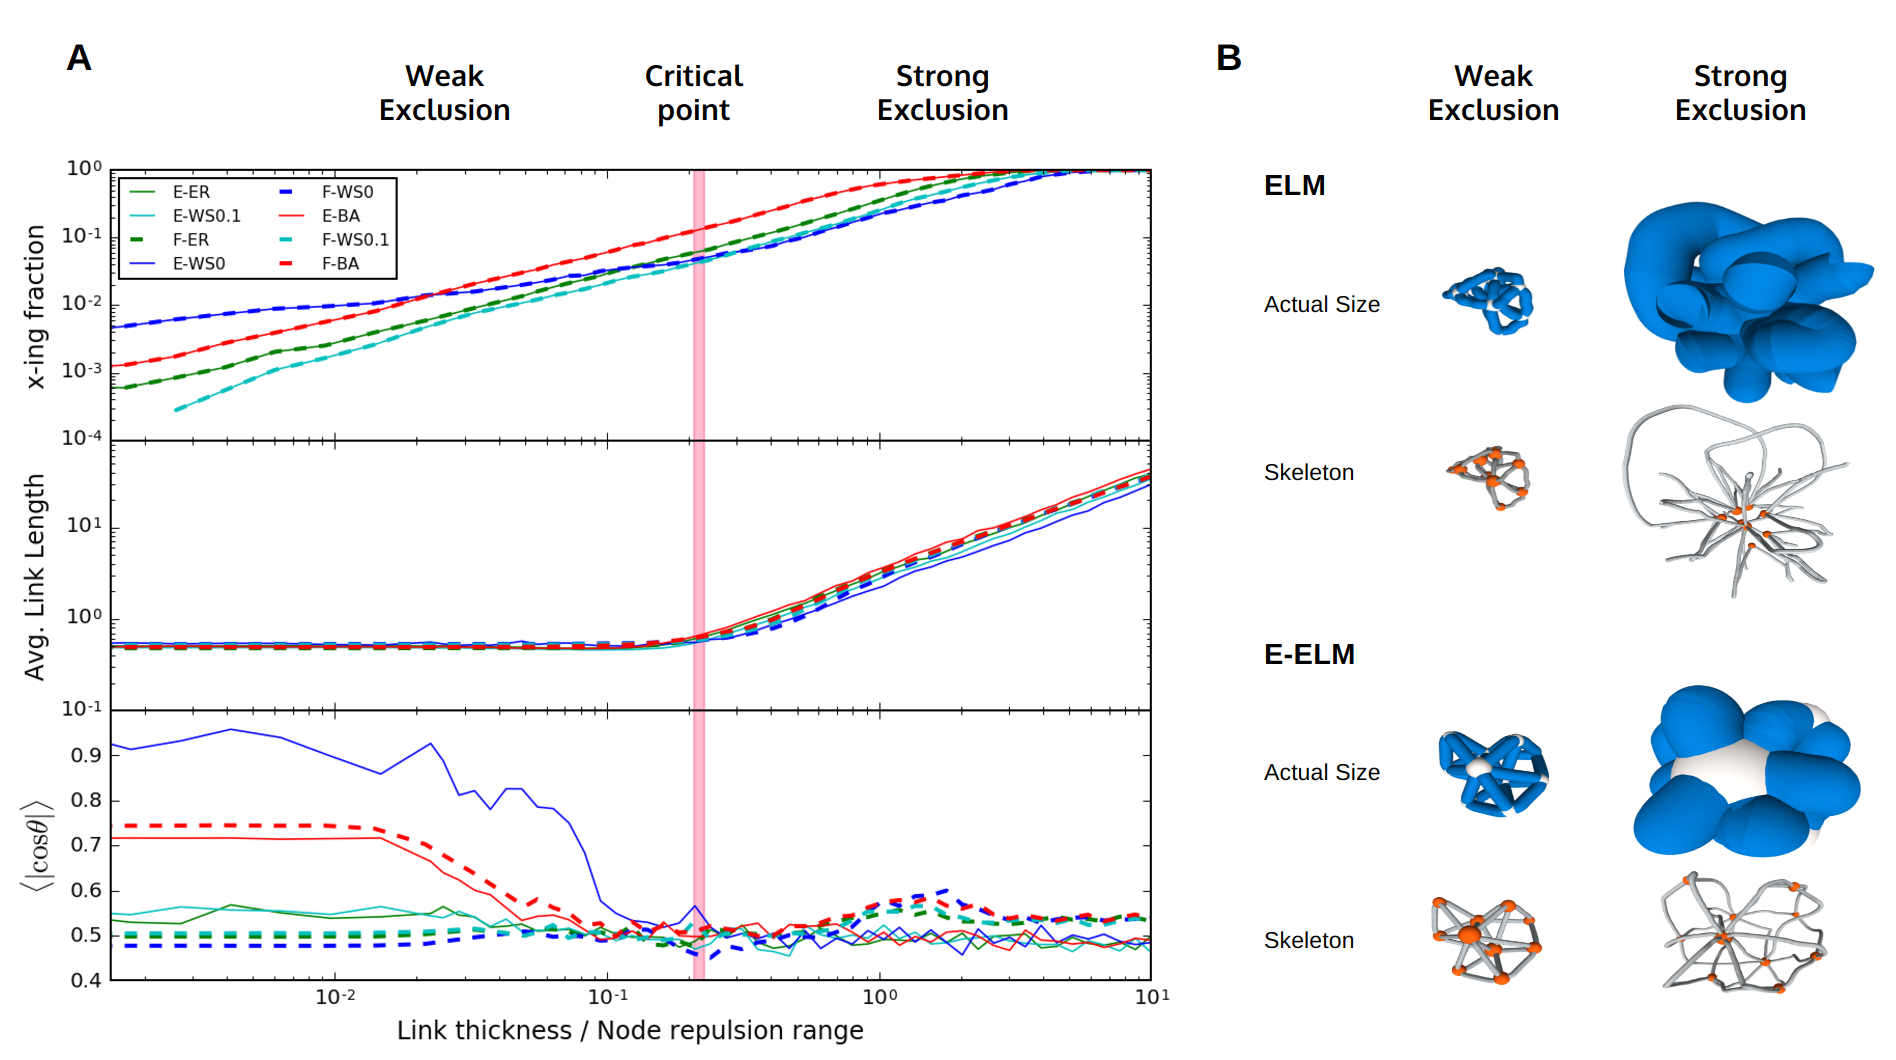
\includegraphics[width=1\columnwidth]{fig-09-19/phase-compare-5.png}
    \caption{{\bf Phases of ELM vs. E-ELM:} Right: Examples of layout in each of the three regions of the diagrams on the left. 
    The first row with blue links shows the actual link thickness, while the second row with gray links is the skeleton to show the paths the links are taking.
    Left: Fraction of crossing links, average link length, average relative angle of adjacent link segments $\be{|\cos\theta |}$, and total tensile stress in nodes and links. 
    Dashed lines correspond to ELM (prefix ``F-'' in legend) and solid ones are E-ELM (prefix ``E-'') layouts. 
    Each color signifies a network topology: ER: Erdős-Renyi; BA: Barabasi-Albert; Lat: the 3D regular lattice. %WS0: Watts-Strogatz with no rewiring; WS0.1: Watts-Strogatz with $p=0.1$ rewiring probability. 
    %In the stress plot, the solid line is the mean stress, averaged over 10 random directions for the compression,  for E-ELM and the shaded area shows 1 standard deviation around this mean. 
    The average link length (second plot) and the total tensile stress build-up (fourth plot) are not good discriminants of different network topologies. 
    Neither does it distinguish between ELM and E-ELM. The $\be{|\cos\theta |}$, on the other hand, does discriminate between both topology and the two layouts ELM and E-ELM in the  ``weak exclusion phase''. In the ``strong exclusion phase'' at large link thickness, however, different topologies laid out using ELM are indistinguishable. Same is true of the strong exclusion phase in E-ELM. %Similarly the strong exclusion phase cannot distinguish topologies in E-ELM. 
    }
    \label{fig:phase-compare}
\end{figure}

Since geometric properties such as average edge length and average angle between adjacent link segments have not been successful in distinguishing between network topologies, we also examine non-geometric measures to check if the strong exclusion phase is indeed universal. We will analyze how different network topologies behave in response to physical stress.

\section{Elasticity and Stress Tensor}
Stress depends on dimensionful parameters such as spring constant of links $k$, link thickness $r_0$ and the range of node repulsion $r_N$, as well as the amount of displacement. 
Stress also depends on the internal structure of the material, which, in our case, is determined by the layout and the topology of the network. 
We investigate whether different network topologies in the weak and strong exclusion phases have different patterns in their stress buildup. 
To understand how ELM and E-ELM respond to stress we must analyze various components of their ``Cauchy stress tensor'' \cite{irgens2008continuum}. 
%Our goal is to find out whether the elasticity and shear stress can discriminate between various network topologies in the weak exclusion and universal phase. 
Consider moving one of a node or a point on a link at position $x$ by a small amount $\delta \vec{x}$.
The network will respond to the change with a force, which to lowest order in $\delta \vec{x}$ is given by
\begin{equation}
\vec{F} (\vec{x}+\delta \vec{x}) \approx %\vec{F} (\vec{x})+\delta \vec{x}\cdot  \vec{\del} \vec{F} (\vec{x}) = 
\vec{F} (\vec{x})-\delta \vec{x}\cdot  \vec{\del} \pr{\vec{\del} v (\vec{x})}.\label{eq:dF}    
\end{equation}
Where $v(x)$ is the potential energy density and the full potential energy $V$ is $V = \int_\mathrm{Net} d^3x v(x)$. 
The term $-\vec{\del} \pr{\vec{\del} v (\vec{x})}$ is the Cauchy stress tensor and has components $T_{\mu\nu}(\vec{x}) \equiv -\ro_\mu\ro_\nu v(\vec{x})$, with $\mu$ and $\nu$ labeling $(x,y,z)$ components. 
Note that $v,F_\mu,T_{\mu\nu}$ are all densities. 
To get the total potential energy, force and stress we need to integrate over the volume of the space. 

In terms of components, we need the Hessian matrix of the potential energy
\begin{align}
    T_{\mu\nu}(x) =&  %\ro_\mu \ro_\nu V(x) =& 
    \ro_\mu \ro_\nu \pr{V_{el}+V_{LL} + V_{NN}+V_\mathrm{end}} \cr
    =& k \delta_{\mu\nu}\int dl \sum_a \delta(x-x_a(l)) \cr
    &+ 
    \sum_{a\ne b} \int \int dl_a dl_b \delta(x-x_a(l_a))\frac{-4r_0^2\delta_{\mu\nu}+ x_{ab\mu} x_{ab\nu}}{16r_0^4}
    A \exp\left[- {|r_{ab}|^2 \over 4 r_0^2}\right]\cr
    &+ \sum_{i\ne j}\delta(x-X_i)\frac{-4r_N^2\delta_{\mu\nu}+ X_{ij\mu}X_{ij\nu}}{16r_N^4}
    A \exp\left[- {| \vec{X}_{ij}|^2 \over 4 r_0^2}\right]
    \label{eq:T}
\end{align}
where $\vec{x}_{ab} \equiv \vec{x}_a-\vec{x}_b$ and $\vec{X}_{ij} \equiv \vec{X}_i-\vec{X}_j$. The first row corresponds to the elastic stress in the links, the second to the link repulsion and the third to node forces\footnote{
Note that the first term contains both the elastic forces and the node-link forces, as they are just the elastic forces at link end-points.}. 
The repulsive terms in \eqref{eq:T} resemble the pressure tensor discussed in \cite{stillinger1984packing} and used for describing jamming phenomena and stress networks in granular material  \cite{o2002random,o2003jamming}.  
Since the repulsive potentials keep links that touch each other at a distance of $2r_0$, we have $\vec{x}_{ab}\approx 2r_0 \hat{x}_{ab}$ if $a$ and $b$ touch. 
Here $\hat{x}_{ab}$ is the unit vector of $\vec{x}_{ab}$.  
If they do not touch, the Gaussian part strongly suppresses the repulsive term. 
Same is true of the node repulsion $V_{NN}$, with nodes that feel each other's force being at a distance $|X_{ij}|\approx 2r_N$ and nodes farther apart than $2r_N$ basically not contributing to $T_{\mu\nu}$. 

In the weak exclusion limit, the stress is dominated by the node terms, i.e. $V_{NN}$ and $V_{end}$. 
In this regime, the links are mostly straight and $\vec{X}_{ij}$ is in the direction of links. 
But the maximum number of nodes surrounding one node is the close-packing ratio in 3D, which is 12. 
To get total stress we have to integrate over $x$, which in the weak exclusion phase translates to summing stress over all nodes.
With the symmetric close-packing, this sum yields $\sum_{<ij>} X_{ij\mu}X_{ij\nu} = \delta_{\mu\nu}$, where $<ij>$ indicates nodes within $2r_N$ of each other. 
But in ransom networks many nodes will not reach this limit and we may therefore have shear (off-diagonal) stress terms.  

In the strong exclusion limit, the links are filling up most of the space in the layout and nodes are more than $2r_N$ apart from each other and so $V_{NN} \sim 0$. 
In the final equilibrium most links are touching other links along their entire length. 
Consequently, around almost all links we have a symmetric enough distribution of other links to get 
%\begin{equation}
    $\sum_{<ab>}\int dl_a dl_b \hat{x}_{ab \mu} \hat{x}_{ab\nu} \sim  N_l\be{l^2} \delta_{\mu\nu}.$ 
%\end{equation}
where $<ab>$ means adjacent links, $N_l$ is the number of links and $\be{l^2}$ is the average square link length. 
The other term in $V_{LL}$ is
$\delta_{\mu\nu}\sum_{<ab>}\int dl_a dl_b \approx N_l \be{l}^2 $
Thus, in the strong exclusion phase the stress tensor should be approximately
\begin{align}
    \int dx T_{\mu\nu} & \approx \delta_{\mu\nu} \pr{k + N_l Ae^{-1} {\sigma_l^2\over 4r_0^2} }
    \label{eq:Tstrong}
\end{align}
with $\sigma_l^2 = \be{l^2} - \be{l}^2$. 
This is a hydrodynamic stress with pressure equal to $ p = k + N_l Ae^{-1} \sigma_l^2 (4r_0^2)$. 
Thus, this approximate calculation suggests that E-ELM results in fluid-like layouts in the strong exclusion limit, while the weak exclusion phase may be more complicated with possible shear stress terms. 
We will examine this claim by only measuring the diagonal terms of $T_{\mu\nu}$ and checking if they satisfy the hydrodynamic conditions of $T_{\mu\mu}=p$ for all $\mu=x,y,z$. 
Measuring shear stress over a heterogeneous structure like a network is not trivial because of ambiguity in what constitutes shear force. 
We will focus on measuring tensile forces, which are what our theoretical calculation suggests is nonzero.  
%Also, to measure total tensile (diagonal) stress, we measure the magnitude of the change in force in all direction in space. 
% the repulsive potential is dominated by links that touch each other. 
% Thus, integrating over the whole space to get total contribution from $V_{LL}$ we get 
% \begin{align}
%     \int dx \ro_\mu\ro_\nu V_{LL}(x) & \approx {A L\over {4r_0^2e}}\sum_{<ab>}  \pr{-\delta_{\mu\nu}+ \hat{x}_{ab\mu} \hat{x}_{ab\nu}}
% \end{align}


% Eq. \eqref{eq:T} can be summarized as 
% \begin{align}
%     T_{\mu\nu} &= \delta_{\mu\nu} \pr{k -{V_{LL}\over 4r_0^2} -{V_{NN}\over 4r_N^2}}
% \end{align}

% To define stress, we need to define surfaces enclosing the network. 
% Forces normal to these enclosing surfaces constitute the diagonal components of stress $\sigma_\mu (x)\equiv T_{\mu\mu}(x)$, or ``tensile stress'' at point $x$. 
% Components tangent to the surfaces make up the off-diagonal components  $\tau_{\mu\nu}(x) = T_{\mu\nu}(X)$, or ``shear stress'', with $\mu \ne \nu$. 
% Since the network is a finite-size, heterogeneous material it is not clear what we should define as the surface. 
% A systematic way for defining shear and tensile stress could be defining the surface as a sphere centered at the center of gravity of the network.
% This way, tensile stress would be all the forces normal to the sphere when the network is compressed in the radial direction.  
% To do this systematically for the whole layout, we choose the surfaces to be 
% We will focus on tensile stress, which are the diagonal components of stress . 
 
To measure tensile stress, we put the networks between two walls, restricting them in a single spatial dimension (Fig. \ref{fig:stress}). 
\begin{figure}
    \centering
    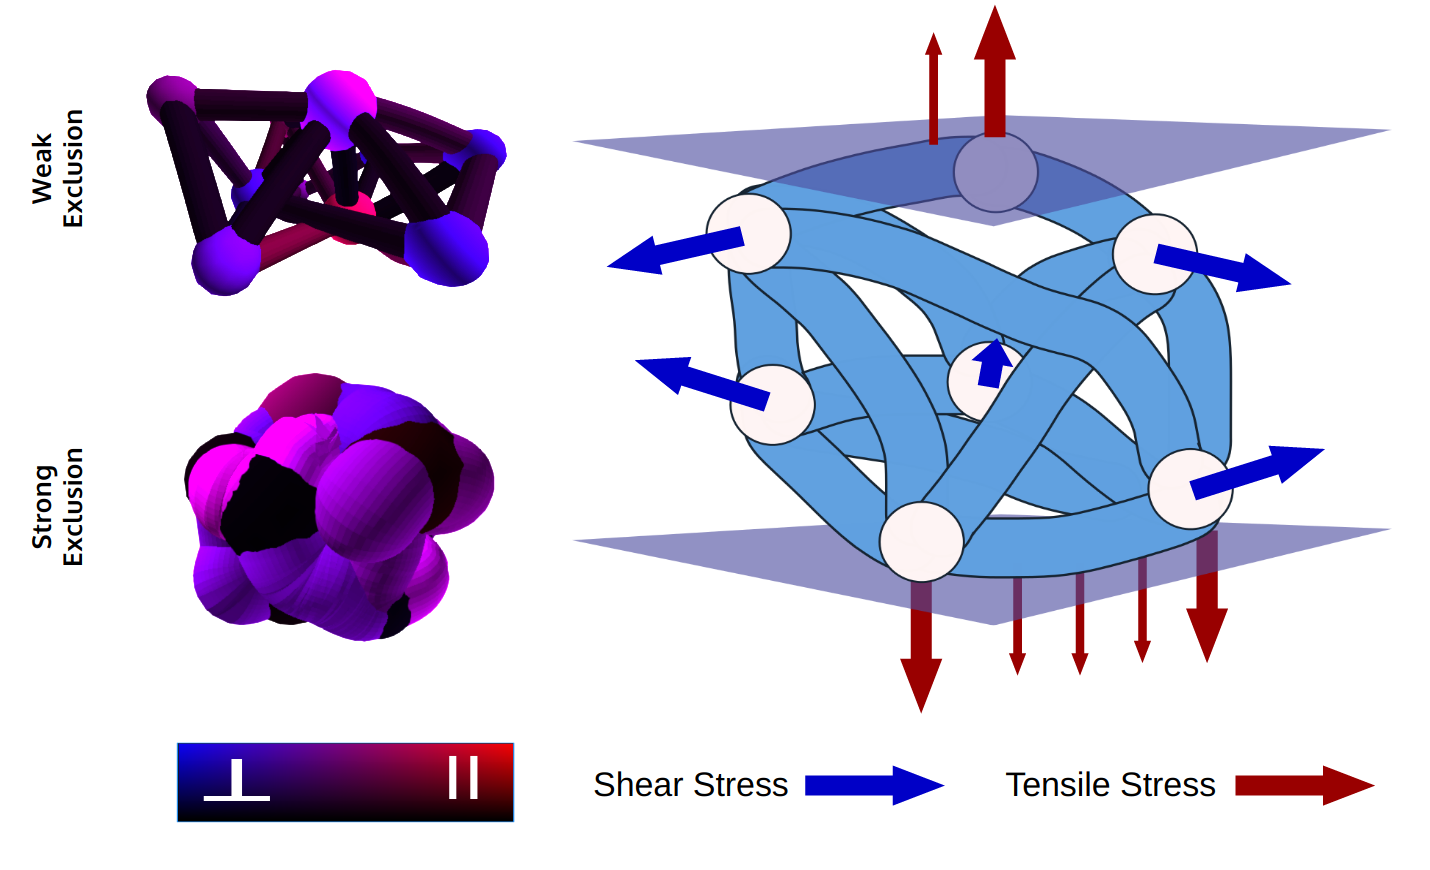
\includegraphics[width = .7\columnwidth]{fig-09-19/stress-ex.png}
    \caption{Right: A sketch of tensile stress build-up in a network as a result of confinement between two walls in the vertical direction. 
    The walls have compressed the network in the vertical direction by a small amount. %$\delta \vec{x}$. 
    The red arrows show the node (thick) and link (thin) forces pushing vertically on the walls.  
    These make up the component of local tensile stress which is parallel to the direction of compression. 
    We denote this by $\sigma_\parallel(x)$. 
    Blue arrows indicate the tensile stress in directions 
    %local shear stress $\tau(x)$ in nodes, i.e. stress 
    transverse to the direction of compression (for clarity, link transverse stress is not shown).
    Left: Examples of tensile ($\parallel$, red) and transverse ($\perp$, blue) stress in networks in the strong exclusion (top) and weak exclusion (bottom) phases. 
    The mixture of blue and red indicates the relative magnitude of the parallel and transverse tensile stress respectively. Darker means smaller total stress. 
    In the strong exclusion phase, all links show stress, whereas in the weak exclusion phase only a few have significant stress. 
    The strong exclusion phase shows more parallel tensile stress at the walls and more transverse stress in the mid parts. 
    The weak exclusion phase, on the other had, shows mostly tensile stress in links, mostly due to change in their length via the compression.}
    \label{fig:stress}
\end{figure}
%Note that since the potential energies among all elements (i.e. link-link, node-link and node-node) in our models only depend on the distance between elements, and because we do not have any dissipative forces, 
%{\color{red} Since a network is like a composite material rather than a single rigid body, the stress properties should be examined using parameters useful for such material. For tensile stress there is no ambiguity, but components of stress that are not in the direction of the displacement manifest themselves in two different ways. In the plane of the confining walls, the stress component normal to the plane is tensile stress and the other two components are shear stress. Everywhere else in the network, the components perpendicular to the displacement become bulk stress components. Thus equality of the magnitude of average stress vectors in all all three directions indicates hydrostatic properties, or that the material behaves like a fluid.}
As described under \eqref{eq:dF}, Stress is basically the change in forces
\footnote{Although formally, it requires defining surfaces and measuring components of force normal or parallel to the surface, since we only want the total stress that builds up in the network we simply measure the changes in internal forces in the layout as a result of compression.}.
These forces yield 
% Stress is defined via defining surface elements and finding the components of force relative to the surface normal. 
% So, in order to measure stress, we will measure the force in link segments and nodes at hypothetical surfaces with normals along $x,y,z$ and with positions crossings various parts of the network. 
% The forces along the normals yield 
the  diagonal elements $ \sigma_\mu \equiv T_{\mu\mu}$. 
The trace  is related to pressure $\sum_\mu T_{\mu\mu} = 3p$. 
Moreover, if the three diagonal  components $T_{xx}, T_{yy}$ and $T_{zz}$ turn out to be similar, the network is showing a characteristic of hydrodynamics. 
% In particular, if the off-diagonal terms are much smaller than $T_{\mu\mu}$ the network is only exhibiting ``hydrostatic stress''.
% Since the potential energy in all elements in the network only depends on distances, none of the forces have components parallel to the surface of nodes or links. 
% This means that stress at any surface will never have shear components (i.e. components parallel to the surface). 
% Consequently, the stress tensor can only have diagonal components.

% Based on the argument above,  only have 3 non-zero stress elements in this model, namely the diagonal terms $ \sigma_\mu \equiv T_{\mu\mu}$. 
Thus, in practice, according to \eqref{eq:dF}, we only need to measure the change in forces throughout the network after compressing the network in one direction by a small amount. 
In the following experiments we compress the networks in the $y$ direction by $5\%$ of their height. 
Since the definition of $x,y,z$ is frame-dependent, we rotate the network 10 times randomly in space to randomize the orientation. 
We will break the tensile stress down into two components: parallel to the direction of compression, $\sigma_\parallel$ and transverse to it $\sigma_\perp$. 
If the rotation causes a large variation in the stress in one direction, for example in the direction of the compression, it indicates that the network has different elastic moduli in different directions and it is not in the hydrostatic regime. 
If, on the other hand, the three stress components $T_{xx}, T_{yy}$ and $T_{zz}$ all have the same magnitude, like hydrostatics, the root-mean-square should obey
\begin{align}
\be{\sigma_\parallel} &={1\over L^3} \int_\mathrm{net} d^3x |\sigma_y| = p\cr
\be{\sigma_\perp} &= {1\over L^3} \int_\mathrm{net} d^3x \sqrt{\sigma_x^2+ \sigma_z^2} = \sqrt{2} p \label{eq:sigp}   
\end{align}
and as a result $ \sigma_\parallel/\sigma_\perp = 1/\sqrt{2}$. The integral is over the volume of the layout and $L^3$ represents total layout volume. 
\begin{figure}
    \centering
    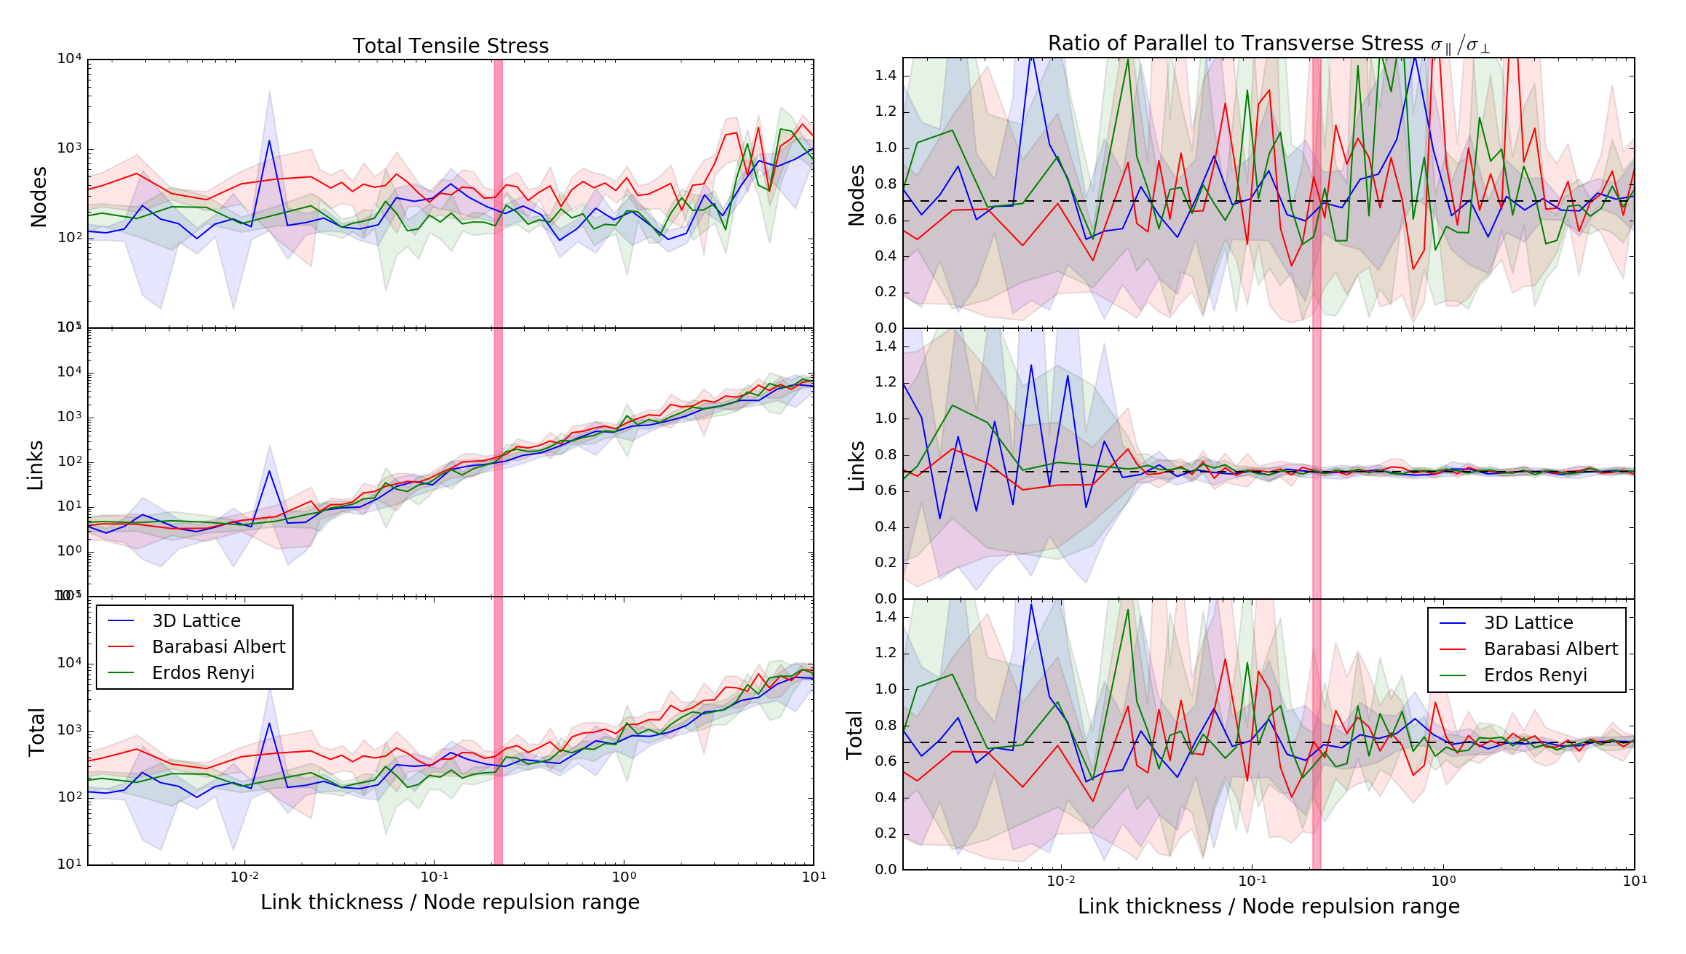
\includegraphics[width=1\columnwidth]{fig-09-19/stress3.png}
    \caption{Left: Total stress in an ER and a BA network with 49 nodes and 280 links, and a 3D lattice network with 300 links at various link thicknesses. 
    The solid curve is the average over 10 measurements done by randomly rotating the layout in space and the  shaded area shows one standard deviation around this average value. 
    The red strip indicates the approximate transition point. % (the lattice has been scaled to match the other two). 
    %The black dashed line is a linear fit to the total stress. It also fits very well with the link stress in the strong exclusion phase, which is because in this phase link exclusion dominates over node repulsion.  
    Right: The ratio of parallel and transverse stress in BA, ER and 3D lattice. In the strong exclusion phase, the ratio becomes $1/\sqrt{2}$ (black dashed horizontal line) in  all three networks. 
    This indicates transition to hydrostatic stress, meaning that stress is uniformly distributed in all direction like a fluid. 
    The green strip indicates the transition point.}
    \label{fig:stress2}
\end{figure}
We examined whether this ratio is satisfied in our layouts by first measuring stress in nodes and links separately and then calculating the total stress in the network. 
We find that for nodes, links and the total stress, rescaling the transverse stress to $\sigma_\perp/\sqrt{2}$ makes the curves of parallel and transverse stress fall onto each other (Fig. \ref{fig:stress2}, left). 
But closer examination shows that the ratio $\sigma_\parallel/\sigma_\perp$ is not constant at all thicknesses. 
We observe that  $\sigma_\parallel/\sigma_\perp$ fluctuates a lot for node stress at almost all (except at very high) link thicknesses, indicating that it does not satisfy the hydrostatic condition (Fig. \ref{fig:stress2}, right, top).
In contrast, the stress in links shows a remarkably constant  $\sigma_\parallel/\sigma_\perp$ ratio starting at thicknesses well below the phase transition, indicated by a red strip (Fig. \ref{fig:stress2}, right, middle). 
At very low thicknesses link stress too shows large fluctuations. 
And finally, when we add the node and link stress, the total stress shows large fluctuations before the transition point, but the fluctuations become much smaller after the transition and the ratio  reaches the $\sigma_\parallel/\sigma_\perp = 1/\sqrt{2}$ hydrodynamic ratio (Fig. \ref{fig:stress2}, right, bottom). This observation, which confirms our theoretical calculation, leads us to the following conclusion: In the strong exclusion limit, networks behave like a fluid. 

Up to this point we still haven't found any order parameter which distinguishes between network topologies in the strong exclusion limit and have found that this phase is quite universal. 
Since topology determines details of how nodes connect, similar to crystal structure, we need to resort to order parameters that are related to the distribution of quantities in the network. 
Thus, in addition to total stress, we will examine the distribution of stress in the layout. 
One observation that we make is that in nodes, stress correlates significantly with degree (Fig. \ref{fig:stress-k}). 
\begin{figure}
    \centering
    \vspace{10cm}
    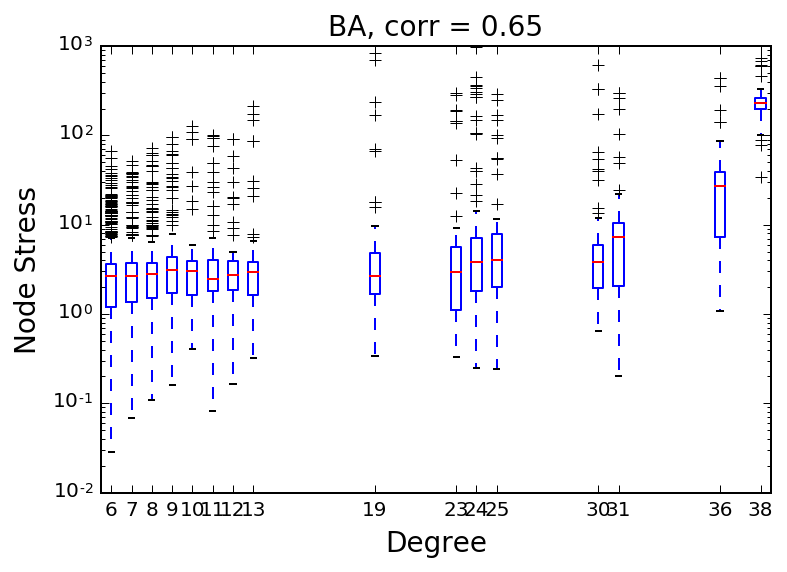
\includegraphics[width=.4\columnwidth]{fig-09-19/stress-deg-ba.png}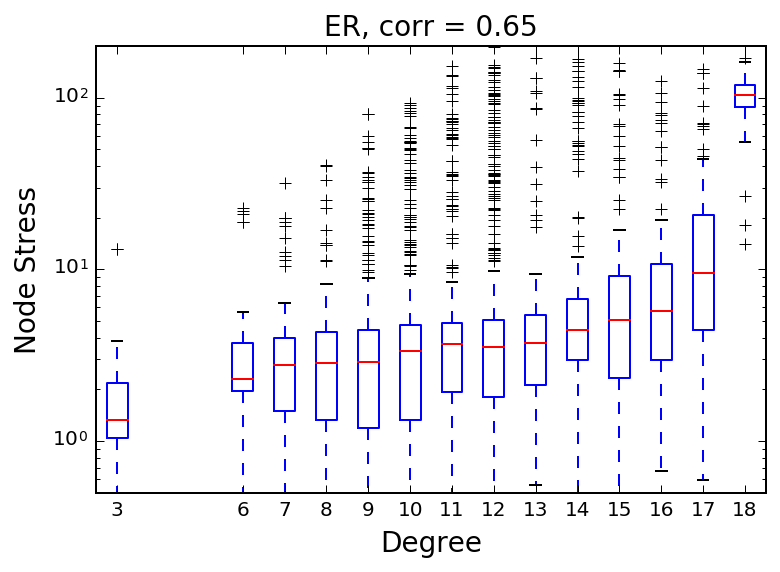
\includegraphics[width=.4\columnwidth]{fig-09-19/stress-deg-er.png}
    
    \caption{Distribution of stress in nodes vs. degree in BA (left) and ER (right), oth with 49 nodes and 280 links. The spread is from layouts at different thicknesses. The Pearson correlation between degree and node stress is 0.61 in BA and 0.58 in ER.}
    \label{fig:stress-k}
\end{figure}
Therefore, just as each topology has different degree distribution, the distribution of stress inside them may be different. 
In light of this, we examine the characteristics of distribution of forces in the two regimes for different topologies. 
We find that, there is a qualitative change in the distribution of forces between the weak and strong exclusion phases (Fig. \ref{fig:Tdist}). 
\begin{figure}
    \centering
    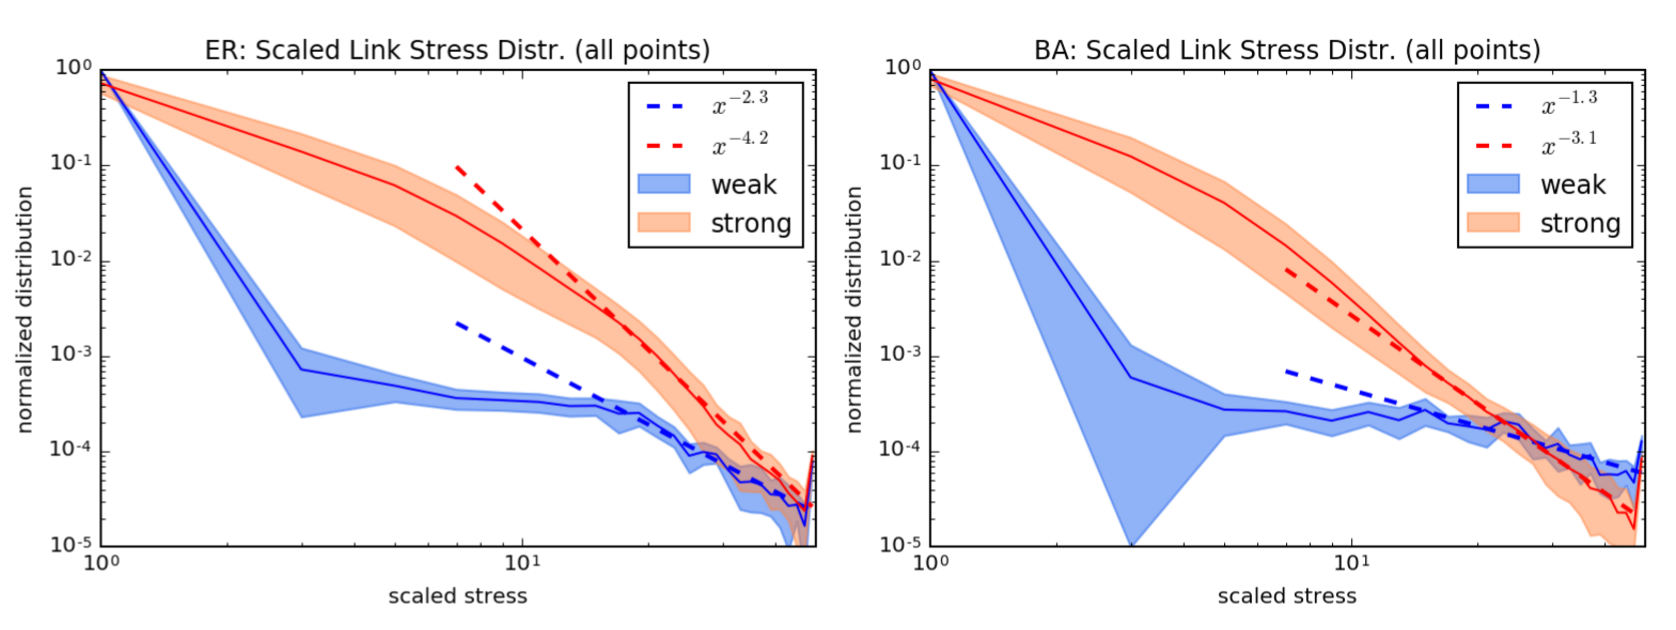
\includegraphics[width=1\columnwidth]{fig-09-19/stress-dist.png}
    \caption{Distribution of stress along links in the weak (blue) and strong (orange) exclusion phases. Left is in ER and right is in BA. }
    \label{fig:Tdist}
\end{figure}
In both BA and ER in the weak exclusion phase, most link segment have no stress in them (the peak of the blue curve at small stress).
Also, in the strong exclusion phase, both show an approximate log-normal distribution. 
But upon closer examination, we found the tails of both weak and strong exclusion limit may be power laws. The exponent for the strong, as well as the weak, regime of ER differs from the exponent of BA. 
This exponent is thus far the only discriminant that we have found for distinguishing topologies in the strong phase. 
But its accuracy and whether it only depends on the topology needs further investigations. 
Additionally, measuring such exponent requires measuring details of stress build-up which is even more involved than simply measuring the degree distribution itself to determine network topology. 
So it is not a useful, macroscopic measure for identifying the topology.



\outNim{
The stress tensor $T_{\mu\nu}$ is symmetric and has 6 independent components. 
Inside the planes of the constraining walls, the stress can be broken into two parts: 
%We compute stress in two forms: 
(1) tensile stress $\vec{\sigma}(x)$, parallel to the displacement $\delta \vec{x}$;  
(2) shear stress $\vec{\tau} (x)$, transverse to $\delta \vec{x}$. They are defined as
\begin{align}
    \vec{\sigma}(x)& \equiv \pr{\delta \hat{x}\cdot T(x) \cdot \delta \vec{x}} \delta\hat{x} \cr
    \vec{\tau }(x)&\equiv \delta \hat{x}\times (T (x)\cdot \delta \vec{x}) 
\end{align}
where $ \delta \hat{x}$ is the unit vector of $\delta \vec{x}$.
%}%%%%% 


Near the constraining walls there will be a higher concentration of tensile stress parallel to the displacement by the , while the periphery and the mid parts of the network will show more shear stress (Fig. \ref{fig:stress}).
In the weak exclusion phase, the layout size is maintained by the repulsive force of nodes.
Therefore stress is much more prominent in nodes (Fig. \ref{fig:stress}, left, top). 
In the strong exclusion phase, link repulsion is dominant and, therefore, stress builds up in links rather than nodes (Fig. \ref{fig:stress}, left, bottom).


\outNim{
Shear stress, technically, refers to stress in the plane perpendicular to the displacement vector $\delta{\vec{x}}$. To speak of stress in locations other than the surfaces touching the constraining walls, we have to consider other components of the stress. Stress components 

What's the problem? We want to measure all forces building up everywhere in the network after pressing it in one direction. Since we haven't yet moved anything except the parts pressed by the walls, there shouldn't be any stress deep in the network. So why do we observe change in forces everywhere in the network? But all we are doing is recalculating the forces and subtracting the original forces. So, maybe the force is indeed zero deep in the network and the contributions are only from the constrained parts. In that case, we really only need the tensile and shear stress at the walls. And there won't be isotropic stress. Of course because the system is static all forces eventually cancel. But we may still measure stress buildup by taking rms values. But how do we interpret the values of the forces we observe all over the network? In particular, which components of the stress tensor do they refer to? If it was uniformly spread over the network we could treat it as overall stress as in continuum limits. But even in that case, which components are they? Tensile stress is obvious, but the components perpendicular to it, are they shear stress or are they diagonal elements, just through other surfaces? If we contain a part of network in a box and measure the stress through different sides of that box, the components which are not immediately at the wall and perpendicular to displacement become diagonal elements of the stress in different directions. But how do we choose these boxes? Also, there will be two vectors, one pushing into the box, the other out of the other side, for every two parallel faces of the box. If we add stress from two boxes with a shared face, that face will cancel, thus leaving us with just the stress on the outer surface of the network. So, how do we quantify local stress trapped inside the network and how does that relate to the conventional stress components? We are measuring the gradient of forces, comparing forces before and after the displacement. Does that relate to stress buildup? It measures the change in internal forces everywhere in the network, but does not necessarily have the same meaning as ordinary stress. Again, how do you quantify something that is related to many components in an object that has many elements? In a rigid body we can use Newton's third law to say that the elements push against each other and that we can use Gauss's law to argue that all forces get transferred to the surface. But when speaking of stress buildup we are assuming non-rigidity.
since our equation of motion is first order, the forces are directly proportional to how much the points in the network would be displaced. Since these displacements are relative to the equilibrium positions, the restoring force will be the second derivative of the potential times displacement squared and corresponds to a spring force.  
We can measure the energy stored in the network. This will be equal to the square of the  
}

We define the total tensile stress, $\sigma$, and shear stress, $\tau$, by integrating these two over the network. %For $\sigma$ we are only interested in the push against the walls and will therefore integrate over a box which presses on the network from top and bottom, but doesn't push on the sides. 
The Young's modulus of elasticity, $Y$, and the shear modulus $G$ for the whole network  are given by 
\begin{align}
    Y &\equiv \frac{\sigma}{ |\delta \vec{x}|/L} &
    G &\equiv \frac{\tau}{ |\delta \vec{x}|/L} 
    \label{eq:YG}.
\end{align}
For $\be{|\sigma|}$ we only use the pressures at the constraining walls\footnote{Distance from walls chosen to be within $(0.01) L$ of the height $L$ of the layout. 
We subtract the push against upper wall from the lower to find total push. }.  
$\sigma = \int d^2x |\vec{\sigma}(x)|/L^2 $, ($L$ being the radius of the layout) but for the shear stress we measure all the stress built-up in the network $\tau = \int d^3 x |\vec{\tau}(x)| /L^3$. 

We evaluate the stress by compressing the layouts by 10\% in random directions $\delta \hat{x}$ and measuring the average quantities $\sigma$ and $\tau$. We find that the ratio $G/Y \approx \sqrt{2}$ (see SI sec. \ref{ap:elasticity} which imlies that all components of $T\cdot \delta\hat{x}$ had the same magnitude. 
Thus, Young's modulus, $Y$, is the only independent quantity regarding the elasticity of the ELM and E-ELM layouts. 
Since keeping nodes fixed when compressing the network interferes with measuring elasticity, we only report the stress build-up in E-ELM (Fig. \ref{fig:phase-compare} left bottom). 
The average of the tensile stress build-up measured over 10 random orientations and its standard deviation show that all three  network topologies BA, ER and 3D lattice have indistinguishable elasticity moduli (Fig. \ref{fig:phase-compare} left bottom). } %%% outnim 030617


In conclusion, we find that in the unrestricted model, E-ELM, the strong exclusion phase (large $r$) is quite universal, meaning all topologies have the same average link length, relative link orientation and even response to stress. 
Indeed, the network parameters, i.e. number of nodes and links, are the only factors that characterize the volumetric properties of these networks. 
This suggests that, if the only constraint is minimizing the volume, then no matter how complicated a network topology is, for a fixed density, the phase diagram of average link length should look the same as what we have derived\footnote{
It remains to be checked how network density would affect the outcome and whether going to lower densities would lead to layout properties that differ among different topologies in the strong exclusion phase.}.
We also find that the universal (strong exclusion) phase behaves like a fluid under stress, whereas the weak phase does not.   


\outNim{
%$F_\parallel/A_\mathrm{N}$ 
divided by fractional displacement
% \begin{equation}
%     Y \equiv \frac{\sigma(x)}{ |\delta \vec{x}|/L} %\frac{F_\parallel/A_\mathrm{N} }{ |\delta \vec{x}|/L} \approx \frac{\int_\mathrm{Wall} d^2x \sigma(x) }{|\delta \vec{x}| L}
%     \label{eq:Y}
% \end{equation}
with the area $A_\mathrm{N}\sim L^2$ being the cross sectional area of the network. 
Similarly, the shear modulus, $G$, is defined by integrating $\tau(x)$ over the whole network 
--measuring the total stress $F_\perp$ built up in directions transverse to the displacement-- 
divided by the cross sectional area\footnote{Assuming the layout is roughly spherical.} $A_N$ and fractional displacement 
\begin{equation}
    G \equiv \frac{F_\perp/A_\mathrm{N} }{ |\delta \vec{x}|/L} \approx \frac{\int_\mathrm{N} d^3x \tau(x) }{4|\delta \vec{x}|L}
    \label{eq:G}
\end{equation}
Both $\sigma(x)$ and $\tau(x)$ vary from point to point. 
%We won't let the system relax completely, as we wish to measure the elastic response of the networks. 
For the tensile stress $\sigma$, we will only consider the direct push against the walls by summing $\sigma(x)$ over all $x$ which are very close to the constraining  walls 
For $\tau(x)$, we measure the total $\tau \equiv \int d^3x \tau(x)$, summing over magnitudes of all points in the network. 
}

   
%} %%%% 

\section{Discussion}
We developed a model for network layout in 3D that minimizes the total volume. 
When the node repulsion is a short-range force, we find 2 phases based on average link length and relative link orientations: a weak exclusion phase and a strong exclusion phase. 
We have found that the average link length vs. link thickness has a universal behavior for all network topologies. 
This can be utilized to classify real-world networks. 
Take, for example, the brains of non-primate mammalian species. 
The number of anatomical regions is similar among these species. 
They differ from each other mostly in the number of neurons and sizes of different brain regions \cite{azevedo2009equal, herculano2012remarkable, herculano2014brain}. 
Thus, at the level of connections of brain regions -- as opposed to connections of individual neuron -- these mammalian brains are similar networks, only different in the thickness of links. 
These links 
%(i.e. bundle of neurons connecting one region to another).
between brain regions, will be bundles of myelinated white matter axons connecting two regions and their thicknesses are proportional to the number and thickness of axons they're comprised of. 
It has been observed that brains of rodents \cite{herculano2012remarkable} and many other mammals \cite{herculano2014brain} follow isometric scaling laws, except for primates, which follow a different scaling\footnote{In \cite{herculano2012remarkable} it is also reported that the fraction of neurons connecting through the white matter stays almost constant across rodent species, which means that Neuron count is proportional to number of axons between regions. The number of axons and their cross-section determines the bundle thickness.}. 
The volume and area of the white matter, $V_w$ and $A_w$, are related as $V_w\propto A_w^{1.5}$ in rodents, and as $V_w \propto A_w^{1.2}$ in primates  \cite{herculano2012remarkable}. 
%An exponent of $1.5$ is consistent with isometric growth, meaning that the whole shape  uniformly scales with radius from species to species. 
If $V_w \propto r^3$ and $A_w \propto r^2$ we get $V_w \propto A_w^{1.5}$, which happens is in agreement with the observed scaling in rodents
\footnote{This is also consistent with the fact that most rodent brains show only small amounts of folding on the surface and the amount of folding changes very little among species.}. In other words, in rodents we expect the link length to scale as $ \be{l} = V_w/A_w \propto r $, the same as the strong exclusion phase, Fig. \ref{fig:phase-compare}. 
In the strong exclusion phase the link thickness determines the size and when links become thicker the node density decreases. 
In rodents, thickness of axons increases while neuron density decreases, but both of these remain constant in primates \cite{herculano2012remarkable}. 
All these observations point to a relations between rodent brains and the strong exclusion phase, but a definitive conclusion requires analysis of the orientations and $\be{|\cos\theta|}$ of axon bundles.%\footnote{
Note that the relation almost certainly doesn't hold at finer resolutions, such as individual connections of neurons. 
For instance, a large degree of parallelism and bundling has been observed in the brain\cite{le2001diffusion,assaf2008diffusion}, which is absent in the strong exclusion phase. This bundling may arise from axonal guidance in the white matter, not minimizing link length that is the fundamental principle of our model.
%}. 
In the weak exclusion phase, node density is constant and there may be some relations to primate brain, which requires more investigation\footnote{
Unchanging neuron density across primates, the increase in folding for increasing number of neurons, the slow growth of $A_w$ with $V_w$, and the fact that the connections through white matter are 4 times less in primates than in rodents\cite{herculano2012remarkable}, all suggest that in primate brain it is not the thickness of the white matter axon bundles that is constraining the system, but rather the huge number of gray matter neurons. 
This would also suggest that primate brains would not be in the strong exclusion phase but rather the weak exclusion phase. Note that the weak exclusion phase allows more organization and parallelism than the strong exclusion.}.


Finally, our model can be used to construct 3D layouts occupying minimal space. 
It can also serve  as a null model to check how optimized the length of links of a 3D network, such as brains or artificial networks, are. 
By altering the definition  of forces, one can also customize ELM and E-ELM to optimize for other conditions, such as bundling, long-range forces, or varying thickness and sizes for links and nodes. 

\bibliographystyle{plain}
\bibliography{mybib}
\newpage
\newpage


\end{document}

%{\color{red} more sims with WS to see if it smoothly covers the whole range between ER and BA and WS0 (Fig. \ref{fig:phase-ws}).% So far, even very small rewiring leads to loss of the high value of $\cos\theta$ and low entropy.
%}

\outNim{
\begin{figure}
    \centering
    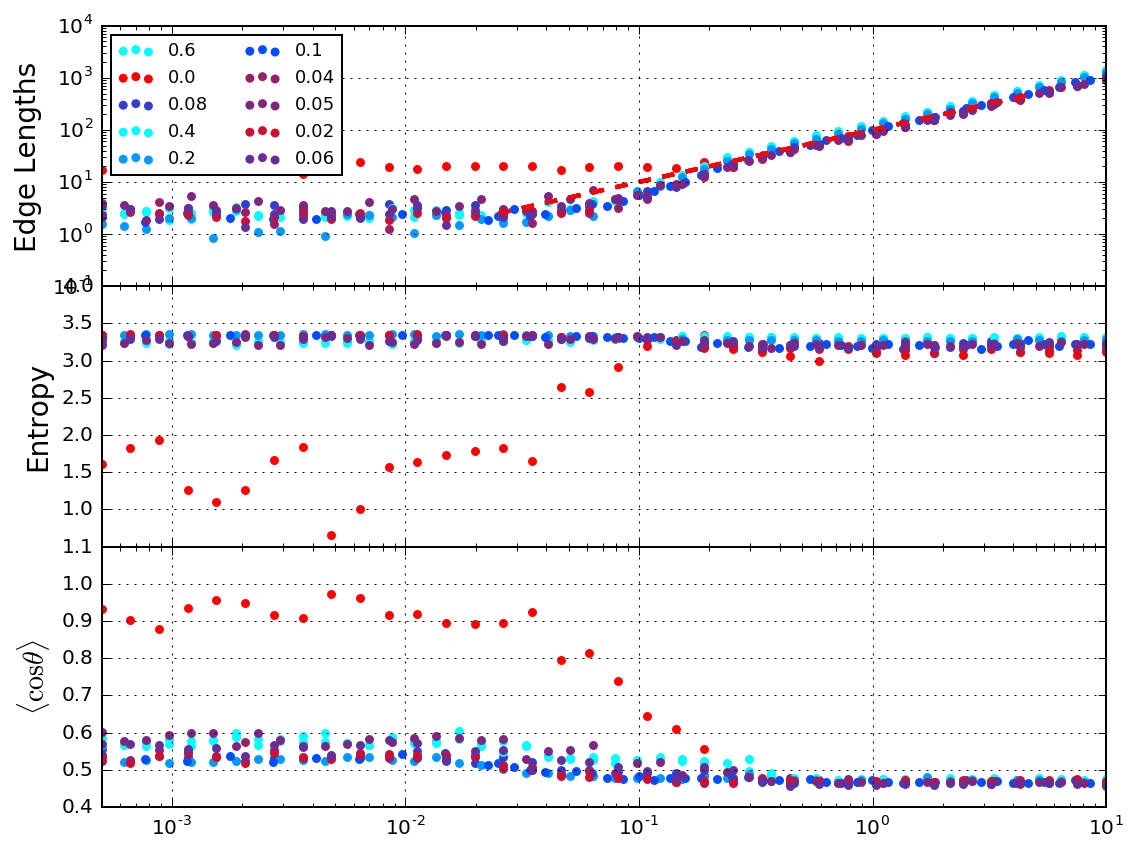
\includegraphics[width = \columnwidth]{fig-09-19/phase-ws}
    \caption{WS with different rewiring probabilities.}
    \label{fig:phase-ws}
\end{figure}
} %%%%


\outNim{
\begin{figure}
    \centering
    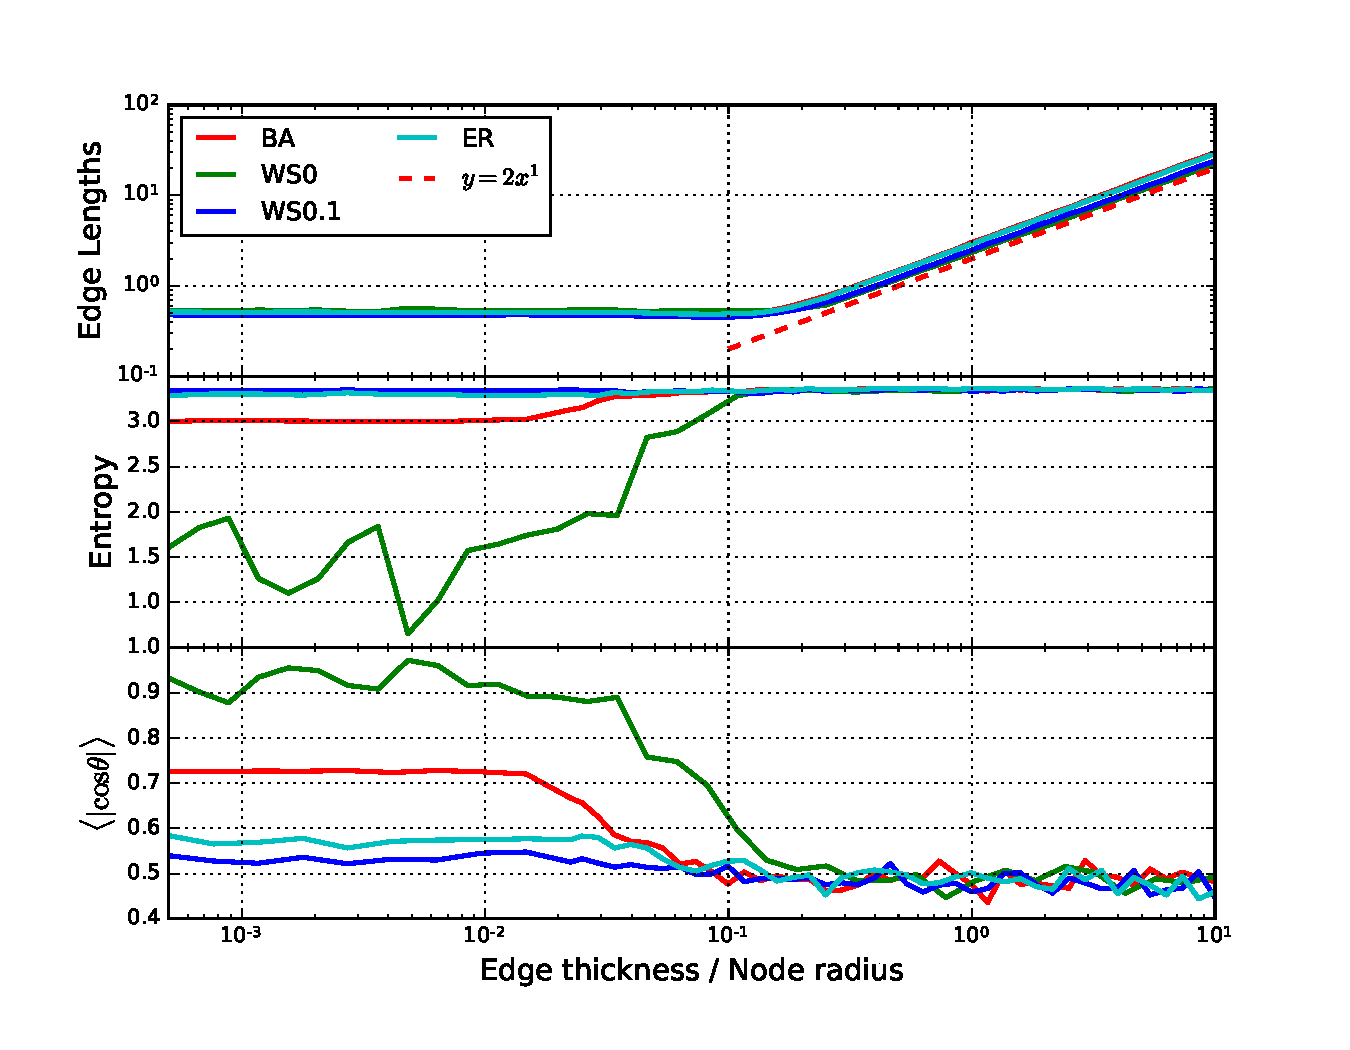
\includegraphics[width=\columnwidth]{fig-09-19/phase-topol.pdf}%phase-eman-all}
    \caption{Comparison of different network topologies. All networks have $N=49$ and $N_e\approx 280$. BA: Barabasi-Albert, ER: Erdős-Renyi; WS0.1: 2D Watts-Strogatz with rewiring probability $p=0.1$; WS0: without rewiring (only with local connections and no small-world property). The top plot shows the average link length. Surprisingly, the average link length is almost identical in all these networks. They all exhibit two phases: one where link length is almost remains constant, happening when links are thin compared to node exclusion radius; and one where average link length grows linearly, suggesting that the layout grows isometrically with the radius. The second plot shows the entropy $S =\sum_n p_n \log p_n$ of the distribution $p_n$ of $\cos\theta$ for angles of segments of eges that touch each other.  }
    \label{fig:phase-topol}
\end{figure}
}%%%

%Fig. \ref{fig:phase-topol} compares these network topologies. % BA: Barabasi-Albert, ER: Erdős-Renyi; WS1: 2D Watts-Strogatz with rewiring probability $p=0.1$; WS0: without rewiring (only with local connections and no small-world property).
\outNim{\color{red}
\textit{Phase transition}. The way links organize depends on the space available for each link. The average length of the links $\langle l\rangle$ is of the order of the network size $L$, combining this with the thickness $r_l$ we get a volume of the order 
$V \sim r_l^2 \langle l \rangle \sim r_l^2 L. $
Thus the maximum thickness $r_{\mathrm{max}}$ would be 
$$ r_{\mathrm{max}} \approx \frac{L}{\sqrt{N_l}}$$
where $L$ is the side of the cube that would engulf the network and $N_l$ is the number of links. Since all links won't organize in parallel, the above condition is a lower-bound on the maximum thickness for which avoiding link crossing should be possible. In practice this yields only the order of magnitude of where we expect a phase transition.

}%%%



\outNim{
\section{Intuition}
In which of the regions should we expect to see the higher brains? Primitive brains have no spatial constraints, especially in non-vertebrates. Now consider the brain of a mammal. The size of the skull is often correlated with the size of the brain. In most animals, it is the cerebellum that contains most of the neurons, unlike human where there are more neurons in the cerebral cortex. 
The growth of the brain and its constraints can be tricky. The skull does not harden completely until most neurons have proliferated and even after neurons stop proliferating, the glia and the brain as a whole grows over time to a few times its original volume throughout the time the animal grows. 
What constraints does that impose? It is not an infinite pressure barrier, but it is also not a free space to roam in. The walls exert a small pressure. The system will have almost minimal volume. The layout of the brain in mammals and birds differ. Birds
do not seem to possess a distinct white matter. Can the restrictions push the system to be at a specific point on the phase diagram? The links will optimize their length as the brain grows. Their thickness will not necessarily fill the volume of the brain. 


\section{Interpretation}
In a biological context, a network scaffolding inside cells, chromatin, or brain cells will generally be inside a container, be it the cell, nucleus, or the skull. None of these containers is completely rigid and in the time-scale of their development, even the skull can thought of as a soft, though somewhat restraining, environment. 

Where would networks inside such soft constraining containers be in our phase space? The container doesn't fully restrict the growth, but it doesn't allow non-economical use of space. How do we quantify this? The container certainly exerts a pressure when the network grows larger. But instead of the pressure growing as the network grows, the container grows with it and it may be exerting a constant pressure on the network. Since elements of the network are elastically repelling each other, to first order the pressure it will exert grows linearly with push in one direction. If the thickness of fibers was growing in the network, they  
} %% outnim


\newpage

%\end{document}

\appendix
{\Huge Supporting Information}


\section{Initial Crossings and Total Volume\label{ap:cross}}
Before examining the bent links, we should first discuss the behavior of link crossing in the embedded network when the link are straight. Simulations using FR confirm that link crossings in this layout behave like random uniform layout of nodes in 3D. It is easy to prove that under such a distribution the number of link crossings grows linearly with link thickness\footnote{Assuming cylindrical links. % with circular cross-section.
}. A sketch helping understand the proof is in Fig. \ref{fig:crs1}. 
\begin{figure}
    \centering
    \includegraphics[width =.99\columnwidth]{figs2/{full-range-n100-m3}.pdf}
    \caption{Left: The behavior of the number of crossings as a function of link thickness. Trivially, once the thickness becomes comparable to the network size (when ``thickness/net. size'' becomes order 1) the crossings saturate and most links cross. The region in which trying to make links avoid each other is much smaller. It extends from zero thickness up to where thickness / net. size is of order $1/\sqrt{N_e}$ with $N_e$ being the number of links in the network. In the BA network with 100 nodes and $m=3$ considered here $1/\sqrt{N_3} \approx 0.06$, which is a safe lower limit for the region where avoiding crossings is possible. Right: a zoomed-in version of the dashed-red box on the lest highlighting this region of validity of avoiding crossings. The legends show a good linear fit to the data up to thickness / net. size = $0.2$.}
    \label{fig:full-range} 
\end{figure}

\begin{figure}
    \centering
    \includegraphics[width =.9\columnwidth]{figs2/crs1.png}
    \caption{\textbf{Left:} The projection of the line through the center of an link \textsf{\textbf{ e1}} on the plane normal to link \textsf{\textbf{ e2}} which crosses the link at point \textsf{\textbf{ n2}}. Because links are randomly oriented, the distance of \textsf{\textbf{ e1}} and \textsf{\textbf{ e2}} is the distance of the blue line from the point \textsf{\textbf{ n2}}. The uniformity then means that the blue lines have uniform density at random angles on the plane and thus their number within distance $d$ is linear in $d$. \textbf{Right:} If links were parallel, the projection of \textsf{\textbf{ e1}} onto the plane would be a point. Thus the distance of the links is the distance of two points on the plane. Uniform spatial distribution in this case means we get uniformly distributed points on the plane and their number within a circle of radius $d$ grows as $d^2$.}
    \label{fig:crs1}
\end{figure}


The key point is that the number of links within distance $r$ of a point on link $a$  can be found by projecting all links onto the plane to which link $a$ is normal. Since the angle distribution is random, we get a uniform distribution of lines on this plane and the number of lines within distance $r$ of a point on a 2D plane grows linear in $r$. 

Analyzing the number crossings as a function of link thickness in FR layout yield a linearly growing number of crossings\footnote{The exact properties of the point where the crossings start is not our primary concern here, but it seems to start at a certain nonzero thickness. 
This sharp phase transition is actually a feature of these connected networks with FR layout. The transition disappears, as expected, in a system of randomly oriented disconnected links in 3D. The length scale at which this phase transition occurs is a function of some dimensionful parameter that can naturally arise from the difference in the form of the repulsive node forces and the attractive forces on the links. We did experiment adding noise to the layout and also randomly switched links around. While these changes increased the slope of the line of the crossings (generally showing more crossings than FR) they did {\em not} move the point of the phase transition appreciably.}. 
%The detailed investigation of the dependence of the phase transition point could be the subject of another work. But 
As far as our goal is concerned, the point where crossings become noticeable seems to depend mostly on the network density parameters, similar to how in self-avoiding polymers the excluded volume depends on the interaction strength. 
After all, the nodes can be modeled as interaction points (vulcanization points) on a self-avoiding polymer.  

% \newpage
% \appendix

\subsection{Examining randomness of crossings}
For simiplicity, let's first consider a number of dots scattered with a random uniform distribution in $d$ dimensional space with a density $\rho$. Suppose we want to grow $d$ dimensional balls around these dots and wish to count the number of balls that overlap. Because of the uniformity, the total number of balls of radius $r$ crossing each other is the number of points that are within less than $2r$ distance of each other, which is
\begin{equation}
    n(r) = \int_0^{2r} \rho(r) dVol=\rho \Omega_{d-1} (2r)^d  \label{eq:nr}
\end{equation}
which scales with the volume of space. In two dimensions, for example, this would mean that the number of circles of radius $r$ crossing each other will be $4\pi \rho r^2$. To compare with the problem of link crossing, if we had parallel cylindrical links in 3d, their cross-section would have been randomly scattered circles in 2D and again the number of crossings should grow quadratically with radius. 

\begin{figure}
    \centering
    \includegraphics[width = .33\textwidth]{figs/para1dir.png}\includegraphics[width = .33\textwidth]{figs/phase-sim-parallel-200-regs-30.pdf}\includegraphics[width = .33\textwidth]{figs/phase-sim-parallel-200-regs-300.pdf}
    \caption{Simulated crossing count of 200 parallel links. One simulation used 30 partition cells in space and the other used 300 cells. In both the number of crossings grows as $r^2$, in accordance with the theoretical expectation. This is in contrast with the linear trend observed in the link crossing of force-directed layouts of random graphs.}
    \label{fig:simpara}
\end{figure}


Now consider infinite cylindrical links scattered with random orientations inside 3D space. Assume that the space occupied by the cylinders has a roughly constant density within cubes of links $d \gg r$. Take the cross-section of this space with a flat plane. The center lines of the cylinders become uniformly distributed points on the plane and the cross-section of the cylinders become ellipses. The ellipses may be very eccentric, but the minor axis, which is also the radius of the largest circle that fits inside the ellipse, is again $r$. Thus, regardless of the eccentricity, if two dots on the plane (the cross-section of center lines of two links) are closer than $2r$ from each other, then the two links will definitely cross. Again, the number of dots less than $2r$ away from each other on any random flat plane grows with $r^2$ and this is only a lower limit for the crossings assuming zero eccentricity for the cross-sectional ellipses.  Therefore the number of link crossings should also grow at least quadratically in 3D.

\begin{figure}
    \centering
    \includegraphics[width = .33\textwidth]{figs/rand-infinite.png}\includegraphics[width = .33\textwidth]{figs/phase-sim-rand-200-regs-100.pdf}\includegraphics[width = .33\textwidth]{figs/phase-sim-rand-400-regs-100.pdf}
    \caption{Simulated crossing count of  randomly oriented links. In both the number of crossings grows as linearly with $r$, in contrast to the parallel link case. This is the same trend as the one observed in the link crossing of force-directed layouts of random graphs.}
    \label{fig:simrand}
\end{figure}

However, contrary to this argument, as Fig. \ref{fig:simrand} shows, the number of crossings among randomly oriented infinite links does grow only linearly with radius, as it did in the random graph layouts. The same linear trend is observed in finite random links.  

\begin{figure}
    \centering
    \includegraphics[width = .33\textwidth]{figs/rand-finite.png}\includegraphics[width = .33\textwidth]{figs/phase-sim-rand-fin-200-regs-400.pdf}\includegraphics[width = .33\textwidth]{figs/phase-sim-rand-fin-100-regs-400.pdf}
    \caption{Simulated crossing count of  randomly oriented finite links which shows the same linear trend as the infinite randomly oriented links, suggesting that the random orientation is cause for the trend.}
    \label{fig:simfin}
\end{figure}



But there are other simpler examples which also show a linear trend in the growth of the number of collisions. For instance, if we take a number of random parallel links and add a similar number of links that go in a direction perpendicular to to those links the trend becomes linear instead of quadratic, as is demonstrated in Fig. \ref{fig:xyz}. The trend is linear for two sets of parallel links, where one parallel set is perpendicular to the other parallel set. The same is true for three perpendicular sets of parallel links. 

\begin{figure}
    \centering
    \includegraphics[width = .33\textwidth]{figs/para2dir.png}\includegraphics[width = .33\textwidth]{figs/{phase-sim-2dir-100-regs-400-rmin=-10}.pdf}
    \includegraphics[width = .33\textwidth]{figs/para3dir.png}\includegraphics[width = .33\textwidth]{figs/{phase-sim-3dir-70-regs-400-rmin=-20}.pdf}
    \caption{Simulated crossing count of 2 and 3 sets parallel links with each set running perpendicular to the other sets. The trend of the number of crossings becomes linear, which is different from the quadratic trend observed in oe set of parallel links in Fig. \ref{fig:simpara} and agrees with the linear trend observed in the link crossing of force-directed layouts of random graphs and in the randomly oriented links in Figs. \ref{fig:simrand} and \ref{fig:simfin}, suggesting that being having components perpendicular to another link may be the key to the linear trend.}
    \label{fig:xyz}
\end{figure}



\subsection{Deriving the linear growth of collisions}
Consider a set of parallel infinite lines distributed uniformly in 2D with linear density $\lambda$ in the direction perpendicular to the lines. Now consider a point $p$ on this plane. The number of links that a circle of radius $r$ centered at $p$ crosses is simply
\[n(r) = \lambda r \] 
and is a linear function of $r$ because only the projection in the direction perpendicular to the lines determines whether or not they cross the circle. 

Now, consider $n$ random lines in a 2D plane with a uniform density (i.e. number of lines passing through a unit square) $\lambda$. Again, the number of lines passing a circle of radius $r$ around a point $p$ grows linearly with $r$. To see this, take a line $l$. Draw the line that passes through $p$ and lands perpendicular to $l$. Say the distance from $p$ to $l$ is $d$. It is only this distance that determines whether or not $l$ crosses a circle around $p$. Because of the rotational symmetry, if we rotate all lines around $p$ and make all lines parallel to each other we will not change the distribution of their distances from $p$. Since they were distributed uniformly in space, the parallel version will also have a uniform distribution. As we showed above, the number of crossings for the uniformly distributed lines grows linearly with $r$ and thus so does the trend for randomly oriented lines. 

The point $p$ in the paragraphs above can be thought of as the cross-section of an link running perpendicular to a plane containing other links. Thus, the number of crossings of an link that is perpendicular to a number of inside a plane, either parallel links or randomly oriented ones, will grow linearly with the radius of the cross-section of links. Thus means that having a number of links crossing planes containing other links leads to the number of crossings becoming linear in $r$. The 3D space can always be stratified in arbitrary parallel planes and as long as there exist a roughly equal number of links going in at least two perpendicular directions, the points found from the crossing of the center lines of an link with a plane containing another set of links always qualifies for the arguments above, even if the link isn't exactly perpendicular to the plane. 

Thus, having links that have components in at least two perpendicular directions in 3D leads to a linear trend in the number of crossings as a function of $r$.  



\section{Minimizing Length and the Stretched Rubber Band\label{ap:affine}}
%#  Numerics of the geodesics
Generally, to find a globally optimum geodesic, be it in flat space or curved space, one has to check many different paths and locally optimize the paths taken. A locally optimized paths, meaning shortest among at each little segement, is a geodesic. But in a non-flat space there exist many geodesics connecting two points. This is because the geodesic equation is a second order ODE and different initial velocities may exist which make the geodesic cross the same final point in space. 



\subsection{The rubber band model}
Denote the components of the metric of the space by $g_{\mu\nu}$. 
Heuristically, since a geodesic is locally the shortest path, a simple way to find geodesics between points should be to assume they are stretched rubber bands. This can be made rigorous. The key point is that For a geodesic we are minimizing the total path locally, which means that we are minimizing the action
\begin{equation}
    S[\gamma;a,b] =\int_\gamma dt \sqrt{ g_{\mu\nu}(x) {dx^\mu(t)\over dt}{dx^\nu(t)\over dt}}  \label{eq:Sdl}
\end{equation} 
where $\gamma$ denotes the geodesic path. The energy for a rubber band is similar, but not the same
\begin{equation}
E[\gamma;a,b]= {k\over 2}\int_\gamma g_{\mu\nu}(x) {dx^\mu(t)\over dt}{dx^\nu(t)\over dt} dt \label{eq:Ekx2}
\end{equation}

%$$ E = {k\over 2} \int_a^b g(\dot{\gamma}(t),\dot{\gamma}(t)) dt $$
But if the parameter $t$ is itself an affine parameter, for example the proper length which is the same as the action $S$ above, we can   show that the equations of motion derived from $S$ and $E$ become the same. To see this, we will derive the Euler-Lagrange equations from varying $S$ and $E$. First define
\[dl \equiv \sqrt{ g_{\mu\nu}(x)dx^\mu(t) dx^\nu(t)}, \]
and for convenience $f\pr{x} \equiv {kx^2/ 2}$ so that $E = \int f(dl/dt) dt $. Varying $S$ yields
\begin{align}
    \delta S =& \int dt \delta \pr{{dl \over dt}} = \left.{\ro \dot{l} \over \ro \dot{x}^\mu} \delta \dot{x}^\mu\right|_{t_0}^{t_f} -\int dt \delta {x}^\mu  {d\over dt} \pr{{\ro \dot{l} \over \ro \dot{x}^\mu}} 
\end{align}
where the first term is a boundary term and vanishes because $\delta \dot{x}^\mu = 0 $ at the boundaries.  
From varying $E$ we have
\begin{align}
    \delta E =& \int dt {df(\dot{l}) \over d\dot{l}} {\delta \dot{l} \over \delta x^\mu} \delta x^\mu \cr
    =& \left.{df(\dot{l}) \over d\dot{l}}{\ro \dot{l} \over \ro \dot{x}^\mu} \delta \dot{x}^\mu\right|_{t_0}^{t_f} -\int dt \delta {x}^\mu  {d\over dt} \pr{{df(\dot{l}) \over d\dot{l}} {\ro \dot{l} \over \ro \dot{x}^\mu}} \cr
    =& -\int dt \delta {x}^\mu \left[ {\ro \dot{l} \over \ro \dot{x}^\mu} {d\over dt} \pr{{df(\dot{l}) \over d\dot{l}}} + {df(\dot{l}) \over d\dot{l}} {d\over dt} \pr{ {\ro \dot{l} \over \ro \dot{x}^\mu}}\right] 
\end{align}
In the last line, if we only had the second term minimizing $E$ would require the same equation as minimizing $S$. The first term here contains 
\[{d\over dt} \pr{{df(\dot{l}) \over d\dot{l}}} = k {d \dot{l}\over dt} ={d^2 l \over dt^2} \]
If the parameter $t$ was an affine parameter, say $ t\propto l$, i.e. proportional to the proper length $l$ itself, this term would be proportional to $d^2 l / dl^2 = 0$  and would thus vanish. So, an affinely parametrized geodesic and the energy function of a rubber band with the same parametrization yield the same equations of motion. Thus, we may replace the problem of finding geodesics between two points with the problem of finding minimum energy configurations of a stretched rubber band connecting the two points. 
%This means that an affinely parametrized geodesic is in fact a minimum energy stretched rubber band. 
The difference in initial velocities of an object following the geodesic, which leads to having multiple geodesics connecting two points, is related to having different spring constants $k$. %Consequently, we will find geodesics by allowing rubber bands to approach their minimum energy states.

\outNim{
\subsection{Other links}

We will implement the curved-space rubber-band similar to flat space. The repulsive force from other links is a function of their geodesic distance, but that is hard to calculate in curved space. Since we assume the force to be short-ranged, we will use a constant metric, based on the midpoint between the two points to calculate the distance between the two points and won't use accurate geodesic distance. 

Also, we will add this repulsive force directly as a force on the l.h.s. of the geodesic equation and won't try to incorporate it into the metric and derive perturbed Christoffel symbols. 
Thus we will only need to define a global metric function.  

}



\section{Contrast with Existing Literature}
The difference between our work and the work of polymer scientists is that we are not concerned with temperature as a parameter. We wish to model phases of the system solely based on total density, i.e. density of links, and the network structure, which determines inter-linkages of links. Again, the motivation is that networks such as brain, or large collagen or polysaccharide fibers in living organisms have very small thermal fluctuations and what we care about is their static properties.

Many aspects of such networks are studied  as part of ``gelation'' processes in polymer physics (see \cite{de1979scaling} chapter IV for instance). Gels are like frozen polymers with inter-linking, like vulcanized rubber. But in polymers the ideal situation with maximally stretched links (occupying minimal volume) is not generally of interest, as it is highly unnatural. For problems such as organization of the white matter of the brain, however, each long fiber has a cost to produce and thus the system may be very economical and make them more efficient.

Physical properties such as stiffness and stress-tensor properties of the network are of course a function of such properties in the link fibers. But these properties will not impact the occupied volume and overall density and thus we are not concerned with them here. 

\section{Methodology}
Our main goal is to understand the volumetric constraints on embedding networks in 3D. To achieve this we will devise a simple model that focuses minimizing the length of links, while avoiding link crossing. For this phase of the work we will assume the nodes are fixed. The layout for the nodes is determined using the popular force-directed layout algorithm Fruchterman-Reingold. 


\outNim{
\begin{figure}
    \centering
    \includegraphics[angle=0, width = .5\columnwidth, trim= 0 0 12in 0 ,clip]{figs1/{sud05}.pdf}\includegraphics[angle=0, width = .5\columnwidth, trim=  11.5in 0 .5in 0 ,clip]{figs1/{sud05}.pdf}
    \caption{methodology}
    \label{fig:forces}
\end{figure}

\begin{figure}
    \centering
    \includegraphics[angle=0, width = .8\columnwidth]{figs1/{sud05}.pdf}
    \caption{methodology}
    \label{fig:forces}
\end{figure}
%} %% out
\begin{figure}
    \centering
    \includegraphics[angle=0, width = .5\columnwidth]{figs1/{method1}.pdf}\includegraphics[angle=0, width = .5\columnwidth]{figs1/{method2}.pdf}
    \caption{methodology}
    \label{fig:method}
\end{figure}
} %% out
\subsection{Elastic Links}
As is known about geodesics \cite{novikov1984} and we also review in appendix \ref{ap:affine} the problem of minimizing the length of links can be mapped to stretching elastic rubber bands between points in space\footnote{The trade-off is that we lose re-parametrization invariance. The energy equation has a fixed parametrization $dl$ which is an affine parametrization of the path.}. The contribution of the stretched rubber band model of link $a$ to the total energy is
\begin{equation}
E_a[\gamma_a] = {k\over 2}\int_{\gamma_a} dl {d\vec{x}_a\over dl} \cdot {d\vec{x}_a\over dl} \label{eq:El}
\end{equation}
where $d\vec{x}_a/dl$ denotes the tangent vector to link $a$ (along the line through the center of the tube), $\gamma_a$ is the path of the link, and $k$ is the spring constant. The energy is obviously a function of the path $\gamma_a$. 

The rubber links will occupy some space and exert a strong repulsive force on each other. Within one link, however, we will only assume no repulsive interactions. This allows the links to shrink to their minimal length under the elastic force of the stretched rubber band model and assume the equilibrium length of the band the be zero to allow for maximum shrinking. 

\subsection{Repulsive force}
We will argue in appendix \ref{ap:repel} that one of the most appropriate choices of repulsive potential which tailored for our purpose is the Gaussian potential. 

We will assume that every line segment in one link has a repulsive Gaussian interaction with every segment of another link. Consider a segment of link $a$. Denote the value of the length parameter parametrizing the path $\gamma_a$ of the link by $l_a$. The tangent vector to this infinitesimal segment $d\vec{x}_a(l_a)$ interacts with segments of other links via
\begin{equation}
dV_{ab} = %|d\vec{x}_a| |d\vec{x}_b| 
dl_adl_b
A \exp\left[- {|\vec{x}_a-\vec{x}_b|^2 \over 4 r_0^2}\right]\label{eq:dVij}.
\end{equation}
Here $A$ is the amplitude of the force and $r_0$ is the cross-sectional radius of the links.  
Thus, the total interaction between segments of $a$ and $b$ is found by integrating over the paths of the two links
\begin{equation}
V_{ab}[\gamma_a,\gamma_b] = \int_{\gamma_a} \int_{\gamma_b} dV_{ab} \label{eq:Vij}
\end{equation}
which depends on the two paths $\gamma_a$ and $\gamma_b$.  

\subsection{Dynamics and Minimum Energy}
In summary, the total potential energy of this system is given by
\begin{equation}
V[\{\gamma\}] = \sum_a E_a + \sum_{ab} V_{ab} \label{eq:V}
\end{equation}
where $\{\gamma\}$ denotes the set of the paths taken by the links. 
To find the ground state of this system, i.e. optimal static configuration, it is helpful to start by introducing the system has dissipative dynamics. This way, instead of having to solve complicated coupled differential equations, we can simulate the dynamics and simply let the system converge to its equilibrium state. 

Consider a point $\vec{x}_a(l_a(t))$ on link $a$ where the length parameter has value $l_a(t)$ and at time $t$. We can introduce a kinetic energy term to the energy which is the sum of the kinetic energies of all infinitesimal segments.
A segment of length $dl$ will have a mass $\lambda dl $, $\lambda$ being the linear mass density, and thus its kinetic energy is
\[dK_a = \lambda dl \left|d^2 \vec{x}_a \over dt \right|^2\]
Summing over all segments we get $K_a[\gamma_a] = \int_{\gamma_a} dK_a$. Friction terms for an infinitesimal segment will have a similar structure. If we assume we are in a viscous medium and that the amount of friction is simply proportional to the length, in the equation of motion a segment of length $dl$, kinetic friction $f_k$ appears as 
\[df_k(l,t) =\eta dl {d\vec{x}_a(l,t)\over dt}\] 
Since the potential depends on both time $t$ and the length parameters $l_a$, the equations of motion are somewhat more complicated than the usual particle equations of motion. We can think of the position vectors $\vec{x}_a (l,t)$ as three component (in 3D) fields whose parameters are $l,t$. The equations of motion are derived the same way as for fields. We have a potential energy density that is a function of both the field $\vec{x}_a$ and its $l$-derivative $\vec{v}_a \equiv d\vec{x}_a/dl$. The equation of motion therefore includes partial integration with respect to $l$. In summary, if we denote components of $\vec{x}_a$ by $x_a^\mu$, we have 
\begin{align}
    \mbox{EoM}:\quad \lambda {d^2 x_a^\mu \over dt^2} +\eta {dx_a^\mu \over dt} & =  -{\ro V \over \ro x_a^\mu} + {d\over dl} {\ro V \over \ro v_a^\mu}   \label{eq:Langevin}
\end{align}
The first term on the right is the familiar $\del_{x_a} V$ and will be nonzero only for the repulsive potential $V_{ab}$. But the second term acts on the internal elastic potential and yields \[{d\over dl} {\ro V \over \ro v_a^\mu} = k {d^2 x_a^\mu \over dl^2}\]  
This is measuring the change in lengths of the segments from one point to another. The reason is that when a rubber band is stretched uniformly, the internal points will not move relative to each other because all forces in all pieces are the same and they cancel out. There will be a non-zero force, and hence movement along the rubber band, only if there is a change in the segment tangent vectors $\vec{v_a} = d\vec{x}_a/dl$ in adjacent segments, as they measure length vectors along the band.


\outNim{
{
\color{red} !!! Needs correction!!!}
\[K_a [\gamma_a]\equiv \int_{\gamma_a} dl \left|d^2 \vec{x}_a \over dt dl\right|^2.\]
} %%%% 
We can now derive the Euler-Lagrange equations for a segment of length $dl_a$ around this point using the action $S = K- V$. To do so, we need the variations with respect to both the position of the points $\vec{x}_a$ and the tangent vector $\vec{v}_a \equiv  d\vec{x}_a/dl_a(t)$. They read 
\begin{align}
%{\delta S \over \delta(d\vec{x}_a/dl_a(t))} : \quad {d^2 \over dt^2 } \pr{d \vec{x}_a\over d l_a} 
{\delta S[\{\gamma\}] \over \delta \vec{x}_a} : \quad {d^2 \vec{x}_a \over dt^2 }  
=&  \vec{\del}_{{x}_a} V[\{\gamma\}]- {d\over dl} \vec{\del}_{{v}_a} V[\{\gamma\}] \cr
=& -k {d^2\vec{x}_a\over dl^2} + {A\over 2 r_0^2}\int_{\gamma_b} dl_b
 (\vec{x}_a-\vec{x}_b)\exp\left[- {|\vec{x}_a-\vec{x}_b|^2 \over 4 r_0^2}\right]
\end{align}
%where we have used 
%\[\vec{x}_a(l_a) = \int_0^{l_a} \vec{v}_a(l) dl  \]

To make the system quickly converge to a local minimum of the potential we will assume strong friction, meaning, if the observation time is $\tau$, we will assume $\lambda \tau \gg 1$ and will discard the acceleration term. So in the end the equation whose dynamics we will simulate to find local minima of this system is 
\begin{equation}
\eta {d \vec{x}_a \over dt }  
= - \vec{\del}_{{v}_a} V + {d\over dl} \vec{\del}_{{v}_a} V\label{eq:Langevin1}.
\end{equation}
Once the dynamics stops, all forces vanish and we will end in some local minimum. 

\subsection{Node repulsion}

To add node dynamics to the system, we will define the node positions $\vec{X}_i$ as dynamical variables. 
The repulsive potential is 
\begin{equation}
V_{ij} = %|d\vec{x}_a| |d\vec{x}_b|
A_N \exp\left[- {|\vec{X}_i-\vec{X}_j|^2 \over 4 r_N^2}\right]\label{eq:VIJ0}.
\end{equation}
where $i,j$ are node indices, $A_N$ is the amplitude of the repulsive potential and $r_N$ is the node radius. 
The force from the links on the nodes does  not come from a new potential. 
It is, in fact, contained inside the elastic potential of the links, %$dV_{ij}$ in \eqref{eq:dVij}, 
as the endpoints of the links is attached to the nodes. The only point is that we will allow nodes to be dynamic, instead of fixed. We denoted tangent vector along link $a$ by $\vec{v}_a(l) = d\vec{x}_a(l_a)/dl_a $. To couple the links with their corresponding nodes we simply need to add a minimal coupling interaction between the end-point tangent vectors $\vec{v}_a (0)$ and $\vec{v}_a (L_a)$ with the nodes they attach to. Here $L_a$ denotes the final value of the affine length parameter $l_a$ for link $a$. The potential for this interaction looks like\footnote{In general each term could have a different coupling coefficient, but that degree of complexity is unnecessary here.}
\begin{align}
   V_{\mathrm{end}} & =c\sum_{i=1}^N \vec{X}_i \cdot \sum_{a\in <i>}  \vec{v}_a\pr{l^{(\mathrm{end})}_a}
\end{align}
where $<i>$ denotes the set of indices of links connected to node $i$ and $l^{(\mathrm{end})}_a$ is either $0$ or $L_a$ depending on which end of link $a$ is attached to node $I$. We will assume $c =1$. We will also assume that the mass and friction constant for the nodes is such that the $\lambda_N$ in the Langevin equation is of the same order as the $\lambda$ for the link segments in \eqref{eq:Langevin0}. 

\subsection{Curse of Local Minima}
Notice that the equations above stop the dynamics at any local minimum. 
Similar to many other coupled systems, such as spin glasses\cite{parisi2002physical,pelissetto2002critical}, the energy landscape of this system is rough and consists of exponentially many locally optimum states which may themselves lie far from the globally optimum configuration. One can   see this fact by assuming a configuration where one link goes around the whole network, instead of going as  straight as possible toward its target. Starting from this situation we can still run the dynamics and shrink all rubber bands as far as possible. The final state is an equilibrium state and a local minimum of energy, but its total energy will be much higher than the global optimum. Therefore, we will use the familiar trick of Simulated Annealing to allow the system to escape local minima and find close-by, potentially lower local minima.  

\subsection{Simulated Annealing and ``vast local minima''}
The trick is to add some thermal noise to the system. In our case, we can think of the thermal noise literally as thermal fluctuations of the links. We start by assuming the positions of link segments are only known as a statistical average and that they fluctuate. Thus we replace

\[dl_a(t) \to \be{dl_a(t)}_{T(t)} \]
where $T(t)$ is the temperature of the system at time $t$. 
The amount of fluctuation will be proportional to the temperature and the energy of the path. Thus, we have to sum over all paths that the links take and we have to weight each path by the Boltzmann factor based the energy of the path. If we discard the kinetic part of the energy because of high friction, the expression for the Boltzmann weight becomes similar to the ``world-line formalism'' of polymers. Denote the sum over all possible paths $\gamma_a$ for link $a$ by $\int [d\gamma_a]$. The partition function for this system, assuming strong friction, is given by
\begin{align}
    Z[\beta] & = \int \prod_a [d\gamma_a] \exp\left[-\beta V[\{\gamma\}]\right]  
\end{align}
with $\beta = 1/T$ as usual. 
This is closely related to the world-line formalism of polymer partition function \cite{des1974lagrangian}. 
Now, instead of the original Langevin equations, the expected values of variables satisfy these equations
\begin{equation}
0= \be{\lambda {d \vec{v}_a \over dt } + \vec{\del}_{{v}_a} V} = \int \prod_a [d\gamma_a] e^{-\beta V[\{\gamma\}]}\pr{\lambda {d \vec{v}_a[\gamma_a] \over dt } + \vec{\del}_{{v}_a} V[\{\gamma\}]}  \label{eq:Langevin2}.
\end{equation}

However, note that this equation only makes sense if we are close to equilibrium because we are using equilibrium Gibbs distribution. That is to say that the thermal fluctuations must happen at a time-scale that is much faster than the time-scale of the dynamics so that the thermodynamic averaging makes sense. When this is not the case, the problem still makes sense as a non-equilibrium system, but the expected value equation above will deviate significantly from zero if the temperature is not extremely small. In other words, even when the dynamics takes the system to the vicinity of a local minimum we have 
\begin{equation}
\be{F(t)}_{T,dt} \approx F \pm \delta t {|\ro_t E|\over \sqrt{T}} \sigma(F)_{T,dt} \label{eq:fluct}  
\end{equation}
where $F$ is the value without thermal fluctuations (i.e. at $T=0$), $|\ro_t E|$ is the rate at which the system's energy is changing. This means that when the system is not at equilibrium the thermal average taken over a period $dt$ will fluctuate in accordance with the rate of energy change. 

%{\color{red} The whole setup of this model is reminiscent of fluctuating manifold model discussed, among others, by Mezard and Parisi \cite{mezard1991replica}}

Since the global minimum cannot be calculated analytically in general, we don't have to worry about near equilibrium description and running the annealing schedule should yield good enough configurations because the fluctuations in \eqref{eq:fluct} allow the system to jump over barriers in the potential energy that are smaller than the $\sigma_F$ term in \eqref{eq:fluct}. 

The setup described above is mathematically similar to that of interacting elastic polymers, or more generally fluctuating manifolds in \cite{mezard1991replica} with imaginary noise and similar problems like the landscape problem, i.e. many local free energy minima, exist here as well. 

\subsubsection{Annealing Schedule}
Then, we start cooling the system with an exponential cooling schedule and once it ``freezes'' as $T \to 0$, we will examine the energy. Simulated annealing is not guaranteed to find the global optimum, but it generally finds states that are much better than a local minimum attained by a fixed initial condition\footnote{ The reason is that the thermal fluctuations allow the system to explore large areas of the energy landscape and the gradient descent introduced as the dynamics will help the system fall into the lowest minimum within that large phase space area. The fluctuations, which allow the system to overcome small barriers between local minima, are effectively smoothening the energy landscape in the sense of \eqref{eq:fluct}. }. This is related to the fact that the thermal fluctuations may be seen as renormalization of the free energy (similar to the discussion of chapter XI of \cite{de1979scaling}) which gets rid of small local dents in the potential energy landscape.  

Thus, all we need to do is add thermal noise to the system during the dynamics and gradually decrease the level of the noise, hence decreasing the temperature and ``anneal'' the system. We choose the schedule of the annealing process to be exponential in time
\begin{equation}
T(t) = T_0 \exp[-t/\tau_{\mathrm{cool}}] \label{eq:coolexp}
\end{equation}
where $\tau_{\mathrm{cool}}$ is the cooling exponent and we choose it based on how fast or slow the dynamics is. The system will need the thermal noise for short period of time. $T_0$ is also chosen based on the parameters of the system. In particular, initially $T_0 > A$ where $A$ is the amplitude in Eq. \eqref{eq:V} of the repulsive potential $V$.   

\section{Simulations}
We wish to examine the effect of network structure on the ``phases'' of the embedded network. The layout of the nodes will of course also affect the volumetric properties. In this work we focus on using the popular force-directed layout algorithm, Fruchterman-Reingold (FR). It ensures that links become reasonably short by assuming they are springs. The angular distribution of the links generally becomes random uniform distribution and thus the algorithm is not biased to organize the network in any way other than the minimized link lengths. This layout assumes straight links and we will bend them to avoid crossings.  


\begin{figure}
    \centering
    \includegraphics[ height = 5cm]{figs1/linkAB}\includegraphics[height = 5cm]{figs1/{linkAB-initial}}\includegraphics[ height = 5cm]{figs1/{linkAB-final}}
    \includegraphics[width = .37\columnwidth]{figs1/{simple3D2}}\includegraphics[width = .4\columnwidth]{figs1/{simple3D}.PNG}
    \caption{result in 3D}
    %\label{fig:my_label1}
\end{figure}


\section{Choosing the Repulsive Potential\label{ap:repel}}

For large molecules one usually uses a potential ansatz like the Lennard-Jones potential $V \sim (r_0/r)^{12} - (r_0/r)^6 $ to simulate the van der Waals interactions, which is weakly attractive at large distances and strongly repulsive at short distances of order $r_m$. Since we are not concerned with molecules here but rather spatially embedded networks in general, we will not assume any attractive force between links and only assume there is a strong repulsion, once link walls get close to each other. The simplest way to model this would be a repulsive force $F = -\del V$ that grows quickly once links get closer than twice the link thickness. In the ideal case, the force is infinite when the two touch or have distance less than twice the thickness. But this force, which comes from an infinite potential, does not behave well for numerical implementation. A remedy is to simply not allow segments to move into each other by fixing minimum distance. But a better strategy numerically is to ``regularize'' the potential by replacing it with a finite potential that achieves approximately the same results. 

The simplest regularization would be to replace the wall potential with a steep incline
\[V \sim \begin{cases} -A(r -r_0) & r< r_0 \\
0 & \mbox{otherwise} 
\end{cases}\]
with $A$ being large compared to $1/\delta t$. 
But again, from the numerical point of view this has the problem that the force is exactly zero at $r_0+\eps$ and nonzero and large at $r_0 - \eps$ which causes numerical error and irregular behavior. Also from the physics perspective this potential is bad because the direction of the force is ambiguous at the origin. A physically meaningful force would either become infinite so that the other particle could never reach $r=0$ or it would go to zero so that the force direction wouldn't matter at $r=0$
\[\mbox{Physical: } \lim_{r\to 0} F(r) = 0 \quad \mbox{or}\quad \infty \]
Since $F(r)\to \infty$ is again numerically ill, the only choice is $F(0) = 0$. To get $F(0) = 0$ we may choose the potential to be an inverted parabola like
\[V \sim \begin{cases} A(r -r_0)^2 & r< r_0 \\
0 & \mbox{otherwise} 
\end{cases}\]
Of course we can also take $V\propto 1/r^n$ %so that the repulsion becomes infinitely large, but that makes numerical simulations harder. One way to resolve that would be to 
and regularize it to something like $1/(r^n+\eps)$, but the resulting force is long-range, because it falls like a power-law. We may again cut this force off beyond $r_0$, but all these choices make the repulsive force harder to control and make assuring that the links stay outside of $2r_0$ distance harder to implement. 

Also, to fix the numerical force discontinuity issue when $r\to r_0$ we have to have a potential which is smooth at $r_0$. Thus instead of the patchwork encountered above, the numerically  sane 
alternative that provides both a controlled, localized force and with an adjustable amplitude without having to patch different functions together and without the need for regularization is the Gaussian potential. %way to implement this without having to use switch cases is to use a Gaussian instead.
The Gaussian provides a force which is smooth everywhere, including at the origin and is therefore an ideal choice for numerical simulations. 
The thickness of the links will then be twice the width of the Gaussian potential and the amplitude is the strength of the repulsion.  

\begin{figure}
    \centering
    \includegraphics[width=.9\columnwidth] {figs2/gauss-pot.pdf}
    \caption{Comparison of the linear incline and the Gaussian potential. While looking similar in shape, the force from the Gaussian is much more well-behaved at $r= r_0$ and $r=0$ and is better suited for numerical analysis. }
    \label{fig:gauss}
\end{figure}


% \bibliographystyle{plain}
% \bibliography{mybib}
\section{ Heuristics} 
This appendix contains some of the  back-of-the-envelope calculations that describe the behavior of the model. 
\subsection{Total link Length Growth\label{sec:growth}}
% Trend of $\Delta $Vol
Assume the length of a segment between a node and another link is $l_0$. Once the other node reaches a thickness $r$ it will stretch this segment to about 
$$ l\approx \sqrt{l_0^2+r^2}$$
when the thickness is smalle compared to $l_0$ so that $r\ll l_0$ we can expand this as 
$$ l \approx l_0+ \frac{r^2}{2l_0}$$ 
So the growth of the total change in link length is 
$$\sum l-l_0 = \frac{r^2}{2}\sum_{l_0} \frac{1}{l_0} = \frac{r^2}{2l_1} $$
As is familiar with resistance of a set of parallel resistors where the total resistance is smaller than the smallest resistance, $l_1 \equiv \pr{\sum_{l_0} 1/l_0}^{-1}$ will be a length scale smaller than the length of any link segment touching two other links or nodes. Thus the mean length divided by total number of links (thus assuming each link is running into all other links uniformly over its path) would be a hard upper limit for $l_1$.
\begin{figure}
    \centering
    % \includegraphics[angle = 0, width = .54\columnwidth]{figs2/phase/{vol-rat}.png}    \includegraphics[angle = 0, width = .45\columnwidth, height=6cm]{figs2/phase/{mean-cos}.png}%{figs2/phase-gen.png}
    
    % \includegraphics[angle = 0, width = .7\columnwidth, height=6cm]{figs2/ER.png}
    \includegraphics[ width = .49\columnwidth, height=6cm]{figs2/vol/{BA-V-crs-n25-m6}.pdf}\includegraphics[ width = .49\columnwidth, height=6cm]{figs2/vol/{BA-V-fit1-n25-m6}.pdf}
    
    \caption{Left: Trend of change in link length $\Delta Vol$ between the bent links (avoiding each other) and the straight links. Right: Total link length growth is consistent with the expected $r^2/2l_1$ with $r$ being the thickness. The length scale $l_1$ is also smaller than the estimated minimum length $min(l)$ of link segments touching other links. }
    \label{fig:vol-crs}
\end{figure}


\section{Force-directed Layout constraints}
We already mentioned that having as much parallel links as possible will make the network more compact. As we increase link thickness we do observe a tendency for links to become more aligned, when they are close to each other. But how does the force-directed FR algorithm perform in terms of efficiently choosing locations of nodes. By it's nature it will take high degree nodes into the center and low degree nodes to the outskirts. What does this mean for efficient use of space? 

A high degree node, such as a hub in BA with $N$ nodes, may have of order $N$ nodes. With link cross-section radius $r$, the radius $R$ of the minimal sphere whose area would completely becovered by the link cross-sections would be roughly 
\[4 \pi R^2 \sim N \pi r^2 \quad \Rightarrow \quad R \sim {\sqrt{N}\over 2} r \]
If this hub node is mall in volume then its links certainly intersect. So, to avoid link crossing at the node the node itself has to be large. The smallest volume it can occupy is when its radius is $R$. This means a hub in BA will occupy about this volume
\[V_{min} = {4\pi\over 3} R^3 \sim N^{3/2} {\pi\over 6 } r^3 \]
Also, we may have at most of order $m$ hubs with degree of order $N$. So in the worst case the volume occupied is of order
\[V_{total} \equiv {4\pi \over 3} R_T^3 \sim (mN^{3/2}) {\pi\over 6 }r^3 \quad \Rightarrow  \quad R_T \sim \pr{m^{1/3} N^{1/2}} {r\over 2 } \]
What if we had allowed the node to be disc-shaped and allowed links to come out perpendicular to it? The area of this disc would be the same as the area of the spherical node, but the links could come out parallel and their length would not be constrained. This means that the volume occupied could be arbitrarily small. Again, we have at most $m$ hubs of degree $O(N)$ and if they are disc-shaped and cover the surface of a spherical area of radius $R_T$, we have
\[4\pi R_T^2 \sim m N \pi r^2\quad \Rightarrow\quad  R_T \sim (m^{1/2} N^{1/2}) {r\over 2} \]
which is larger than the radius for the spherical distribution of links around nodes because in the spherical we allow all links of a node to cross each other and simply make node so large that at its surface there won't be any more crossings. 

% For localized degree distributions like the ER model, we have $O(N)$ nodes all with degree around $m$, but we can't link them straight. The only way to get a good coverage and be able to link the required nodes is to have the nodes distributed rather uniformly on the surface of a shphere. ... this time 
% \[R_T \sim m^{1/2} N^{1/2}\]




\begin{figure}
    \centering
    \includegraphics[width=.4\columnwidth]{figs/eman/eman-100}\includegraphics[width=.4\columnwidth]{figs/eman/eman-100-skeleton}   
    \includegraphics[width=.4\columnwidth]{figs/eman/FR-skeleton}
    
    \caption{Top left: BA $N=100, m=3$ , emancipated nodes with large thickness/node radius ratio. All links are pulling the network together, but there is sufficient space for all and the network is in general under much less stress than the case when the nodes are held fixed. Top right: Skeleton of the same outcome of the layout showing how links are stretched to avoid crossing one another. Bottom. Skeleton of a BA $N=100,m=3$ with fixed node positions layed out using FR and link thickness above the transition point (i.e. not enough space available). links inside the convex hull of nodes cannot avoid crossing. Many links get pushed out of the convex hull and go almost radially outward from the nodes and make long bows to reach their targets.    }
    \label{fig:skeletons}
\end{figure}


%\section{Old}



\section{Finding Overlapping Links}
Consider two straight links $A$ and $B$. Denote the two vectors pointing to the endpoints of the two links by $A_1,A_2$ and $B_1,B_2$. Define the $a= A_1 - A_2$ and $ b= B_1 -B_2$ which are parallel to the lines connecting the two endpoints of each link. The links are cylinders of diameter $d$. We wish to find whether or not the two links intersect, i.e. whether the two links come closer than a distance $d$ of each other. The shortest distance of the two vectors is $a \times b$, since this is perpendicular to both $a$ and $b$. Define
\[c = a\times b\]
we can decompose $ a$ to its components parallel and transverse to $b$ 
\begin{align}
a &= a_\parallel \hat{b}+ a_\perp (\hat{b}\times \hat{c})\cr
a_\parallel &= a\cdot \hat{b}, \cr
a_\perp &= a \cdot (\hat{b}\times \hat{c}) = \hat{c} \cdot (a\times \hat{b})= {|c|\over |b|}
\end{align}

\subsection{Measuring link distance}
Consider the plane $P$ spanned by $b$ and $c$ and containing the link $B$. The unit vectors $\hat{b}$ and $\hat{c}$ form an orthonormal coordinate system for this plane and any point on the plane can be written as
\[x_p = x_b \hat{b}+ x_c\hat{c}\]
The plane itself is defined through the normal vector 
\[\hat{n}= \hat{b}\times\hat{c}\]
and hat multiple $p\hat{n}$ of $\hat{n}$ from the origin intersects the plane.

When $ a$ and $b$ are not parallel to each other, $a$ will cross the plane $P$ at a single point. The projection of link $A$ onto $P$ is a line parallel to $B$. Therefore we can use the following to find the distance between the two links. We will first pick one endpoint from each of $A$ and $B$. The vector connecting the two
\[d = A_1-B_1\]
is a vector whose projection of the vector $c = a\times b$ is perpendicular to both $a$ and $b$ and thus also to the projection of $a$ onto $P$. Since on $P$ the projection of $a$ is parallel to $b$, the magnitude of the projection $d_p$ of $d$ onto $P$ is the minimum distance between the two links. Thus we have
\[|d_p| = d \cdot \hat{c}\]

\subsection{Caveat}
The above mentioned $d_p$ is the least distance of the two links only if $A$ crosses the plane $P$. Otherwise, one of the endpoints will be the closest point to the other line and we need a different strategy. Let's first figure out a way to see if $A$ crosses $P$ or not. To this aim we will look at the projections of $d_1= A_1-B_1$ and $d_2 = A_2 - B_2$ along the normal $\hat{n} $. Regardless of which endpoints of $A$ are being connected to which on $B$, if the projections of $d_1\cdot \hat{n}$ and $d_2\cdot \hat{n} $ have the same sign it means $A$ did not cross $P$ and if they have opposite signs or one is zero $A$ will have crossed $P$. Thus  
\[\mbox{if: } (d_1\cdot \hat{n})(d_2\cdot \hat{n}) >0 \quad \Rightarrow  A\mbox{ not crossing }P\]
And so the closest point on $A$ to $B$ is one of $A$'s endpoints. Similarly, we need to check if $B$ crosses the plane spanned by $A$ and $\hat{c}$. If not, the closest distance of the $A$ and $B$ will be one of their endpoints to each other. 



\section{Estimating the space required}
Consider an unweighted, undirected network visualized in 3D.  
Suppose all links have a cross-sectional radius $ r_e$ and thus an area $a_e = \pi r_e^2$. We may choose the radius of nodes in such a way that its area $a_n$ would be roughly the number of its links  of the total number of links that come out of it. When the degree $k\gg 1$ we have $a_n \approx k a_e$ and so the radius of the node $$r_n \approx \sqrt{k}r_e/2.$$ 

However, when $k$ is small,such as $k =1,2$, the node may be much smaller and the smallest spherical node is such that the cross-section of links with it become one of the great circles of the sphere. This means that 
$$ \pi r_e^2 = \pi r_n^2  \quad \Rightarrow \quad  r_n = r_e.$$
Thus for visibility, we could choose, say 
$$r_n = \sqrt{k} r_e$$
which will make sure the nodes are large enough to be visible for all $k$. 

\outNim{
Experimenting with the size of nodes revealed that instead of taking the area to be proportional to the degree, doing so with the node volume yields better results. This may be because of the following. 

Suppose we have $k$ links of cross-section $a_e$. 
Assume that they are uniformly spread at different solid angles around a center that is the center of the circular cap at one end of them. 
The question is: what is the minimum radius of sphere around the same center which would cross the links in such a way that the cross-section of one link on the sphere's surface would not intersect other links' cross-section. 
Take the circular cross-section of one link with the sphere. Connecting the center of the sphere to this circle yields a cone, whose volume is $h a_e /3$, with $h=\sqrt{r^2- r_e^2}$ being the height of the cone. If the number of links is large and we work with the smallest radius at which links don't intersect, the total volume of these cones will be close to the volume of the sphere, $4\pi r^3/3$. Solving for $r$ yields
\[ {k\pi\over 3} r_e^2 h \approx {k\pi\over 3} r_e^2 r =  {4\pi\over 3} r^3 \quad \Rightarrow \quad r = {\sqrt{k} \over 2} r_e  \]
When $k \gg 1$ The links may cover the surface of the sphere and so $k \pi r_e^2 \approx 4 \pi r^2$, which also yields $r = \sqrt{k}r_e /2$.  
However, when $k$ is small, the volume of the cones is much smaller than the volume of the sphere. In fact for $k=1,2$ the volume of the cones is zero and their cross-section with the sphere becomes one of the great circles of the sphere. This means that 
\[ \pi r_e^2 = \pi r^2  \quad \Rightarrow \quad  r = r_e.\]
} %%% out

\subsection{Theoretical limits on the embedding size}
Take a network of $N$ links and a degree sequence $\{k_1,...,k_N\}$. Define the link radius $r_e$ as the unit length, i.e. $r_e = 1$ Taking spherical nodes of radius $r_a = \sqrt{k_a}$, the volume they occupy is 
\[V \sim \sum_{i=1}^N k_a^{3/2}\]

%If the $N$ and the total degree 
Define $K= \sum_a k_a$. %is fixed, because the volume is a super-linear function of $k_a$, the largest volume will be that of 
Consider 
a uniform network with degrees $k_a = K/N$. In this case the volume is 
\begin{equation}
    V \sim N {K^{3/2}\over N^{3/2}} = {K^{3/2}\over N^{1/2}} \label{eq:uniform}
\end{equation}
whereas in the other extreme, where one node has degree $N-1$ and all the others have degree 1, we would get
\[V \sim N-1+ (N-1)^{3/2} = O( N^{3/2})\]
The smallest connected uniform network is a ring where $k_a=2$ and $K = 2N$. In this case
\[V\sim 2\sqrt{2} N \]
which has less volume than the extreme star-shaped network above. For $k_a = k $ we still have 
\[V \sim k^{3/2} N \]
When $k > N^{1/3}$ this will be larger than the volume of the star-shaped graph.


The densest uniform network is the complete graph with $k_a=N-1$ and $K= N(N-1)$. This yields
\[V \sim N(N-1)^{3/2} \approx N^{5/2}\]
which has a larger volume than the star-shaped graph. 
\subsubsection{Random graphs}
Consider random regular (RR) graphs, where all nodes have the same degree, $k$, and the Erdos-Renyi (ER) graph, where the degree distribution is a Poisson distribution, which approaches a Gaussian at large average degrees. An ER network has a percolation threshold of $k = \be{k_a} = 1 $, meaning that if $k>1$ the network will have a giant component whose size is of order $N$. Since we are considering the embedding of a connected graph, we need the connectedness threshold. For ER this threshold is\cite{erdos1960connected} $k > \ln N$, meaning that the probability of finding isolated links tends to zero. The expected volume for such a network becomes
\begin{equation}
    V \sim O\pr{N (\ln N)^{3/2}}
\end{equation}
Since the ER has a Poisson degree distribution, most nodes have degrees of the order of the average degree $k$. Therefore, we may use the results from the uniform network for estimates with ER as well.  
Above we found that if $k> \sqrt{N}$, the network volume will be larger than the extreme star-shaped graph. Note that for large $N$ 
\begin{align}
    \ln N  = N^{1/3},\qquad 
    y  \equiv {1\over \ln N},\qquad
    %n &\equiv \ln N\cr
    %n &= e^{n/3}\cr
    %\ln n & = {n\over 3}\cr
    %n^{1/n} &= e^{1\over 3}\cr
    y^y = e^{-1/3}
\end{align}
\begin{figure}
    \centering
    \includegraphics[width= .5\textwidth]{figs/log-vs-star.pdf}
    \caption{ER connectedness threshold $k= log N$  versus $K = N^{1/3}$ which is the limit above which the volume of the ER will be larger than the extreme star.  As we see, for $N>100$ an ER at connectedness threshold may occupy less space than the star.}
    \label{fig:logstar}
\end{figure}
This expression has two solutions. The smaller one can be written as 
$$ N = -3 \mathrm{LambertW}\pr{-{1\over 3}} \approx 6.4 $$ 
The larger root is around $N = 94$. Thus for any network with $N >100$ an ER network right at the threshold of connectedness may occupy less space than the star-shaped graph, ignoring space required by links. 

\subsection{The general case}
Consider a network with degree distribution $P(k)$. Ignoring the space required by links, the minimum space occupied by the nodes is 
\[V \sim \int dk P(k) k^{3/2} \]
We heuristically discussed the case of localized, Gaussian degree distributions above. We may use this expression to make the calculations more precise. But first let us solve the much simpler case of Power-Law degree distributions $P(k) \sim k^{-\gamma}$ with $\gamma \geq 1$ and with a max degree $k_{\mathrm{max}} \sim N$. We have

\begin{align}
    V &\sim \int_0^N dk k^{-\gamma +3/2}\cr
    \mbox{if: }\gamma \neq 5/2\quad \to 
    V &\sim N^{-\gamma + 5/2} \cr
    \mbox{if: }\gamma = 5/2\quad \to 
    V &\sim \ln N
\end{align}
Thus, for example the BA model with $\gamma = 3$ yields 
\[V \sim N^{1/2}\]

\section{Phase Diagram of Number of Crossings} 
Let's find the number of crossings as a function of link radius. We will divide this radius by $N^{1/3}$ to get average space per node. The number of links should be of $2N$ because each new node brings in exactly 2 new links. Thus we expect most links to intersect once their radius becomes of order $r/2 $. 
When the thickness is very small we expect there to be very few crossings. In this case perturbing the layout should be able to resolve the crossing. At very high thickness, though we know that the layout may get clogged up so that no perturbation could resolve the crossings. There should be a qualitative difference between these two states.  

\outNim{
\begin{figure}
    {\tiny 
    \begin{tabular}{ll}
    \qquad\qquad BA~(n=200, m=3) & \qquad\qquad BA~(n=500, m=2)\\%[-5pt]
    %{\centering
    \includegraphics[width = .48\textwidth, trim = 0 0 0 1cm, clip]{figs/phase-ba-200-3.pdf}&\includegraphics[width = .48\textwidth, trim = 0 0 0 1cm, clip]{figs/phase-ba-500-2.pdf}\\
    \includegraphics[width = .48\textwidth]{figs/{phase-er-100-0.05-reg-500}.pdf}&\includegraphics[width = .48\textwidth]{figs/{phase-er-300-0.03-reg-500}.pdf}
    %} % centering
    \end{tabular}
    }% tiny
    \caption{Caption}
    \label{fig:phase}
\end{figure}
}
Simulations of Barabasi-Albert and Erdo\"os-Renyi networks layed out in 3D using the Fruchterman-Reingold forced-directed layout seems to suggest that in this setting the qualitative behaviour of these networks for different values of parameters is very similar. Figs. \ref{fig:simpara},\ref{fig:simrand} and \ref{fig:simfin}  shows simulations with parallel, randomly oriented and finite links, respectively. The plateau in the number of crossings at large radii is due to the limitation of the optimized algorithm, which partitions the space into smaller boxes and fails when the link radius reaches box size. 
%Therefore we expect there to be a rather smooth phase transition between the two phases, akin to a second-order phase transition. 
As we can see in Fig \ref{fig:simrand} the number of crossings in both type of networks and in all four simulations grows linearly with link radius. The question is whether this is due to the layouts randomness. 

\section{Optimizations}
Brute-force calculations quickly become intractable for even medium sized networks. We used a number of strategies to optimize these computations. Many of them involve binning the space in various ways to focus only on the parts where computations is required. Such strategies in some cases reduce the computation time by a factor of 10 or more as they change the time complexity of the problem. 

\subsection{Making finding crossings more efficient}
we only need to check pairs of nodes that have a chance of crossing links. That means only nodes $A:(a_1,a_2)$ and $B:(b_1,b_2)$ for which in all three of x,y,z directions they fall within a certian geometric shape. If links were just lines, the suffiecient condition would have been that $A,B$ form a tetrahedron with no obtuse angle. Since we only wish to speed the search for crossings up, we can choose a very crude measure. The constraint is that the measure has be evaluated very efficiently and very rapidly, faster than it would take to do the computation for checking the crossing, which involves calculating 3 cross products and several dot products and square-roots. 
\subsection{ Restructuring accessing links make potentially crossing link look-up more efficient}

What matters is the spatial region from which the links pass through. We will use the link id, based on location in the link list and compile a dictionary of regions in space through which at least one link passes. These regions may be sparse, depending on how their scale compares to the total space occupied by the network. This regional approach allows spotting precisely which segments of which link are crossing. 


If the network has $M$ links,we have to make sure compiling this dict and looking up pairs takes less than $O(M^2)$. If the computations are short, compiling the dict should be $O(M)$. 


\subsection{Breaking space up into regions}
Consider a uniform graph of average degree $m$, and with $k$ cells occupied. We have $M = Nm/2$ links. Each link may stretch several regions. If they stretch $q \ll k $ regions, we will break the links into $q$ segments. The total number segments yields the cumulative occupancy of the $k$ regions. Thus each cell has $Mq/k$ links. The total number of checks for crossing is therefore


$$ O(M) + O(k)+ O\left( k \times \frac{M^2 q^2 }{ k^2} \right)= O(M)+ O(M^2 q^2/k) $$
Assuming the look-up of the dict is $O(k)$. Thus in order for the regions approach to be more efficient than the original we must have a situation in which $q \ll \sqrt{k}$. If our links are straight lines, if the network is embedded more or less symmetrically in all three dimensions, then the maximum number of regions a link may pass through is $O(k^{1/3})$. For $k \gg 1$ a uniform embedding in $d$ dimensions yields 

$$ q \sim O(k^{1/d}) \ll O(k^{1/2}), \qquad \mbox{if: } k\gg1 \quad \mbox{and } d> 2$$ 
And thus in 3D this method will most likely improve the performance. The amount of improvement is
$$ O\left( \frac{M^2 k^{2/3} }{ k} \right) = O\left(\frac{M^2}{ k^{1/3}} \right) $$

Thus the full complexity depends on how many cells we choose. Assuming that look-up of the dict can be done in linear time $O(k)$, if we choose $ k$ such that $1\ll k \ll M$, we can significantly accelerate finding crossings.  

Implementing this resulted in a very significant improvement in finding link crossings. For a BA network of 500 links and $m=2$ minimum degree, the brute force method took about 20secs, while the regioned approach with maximum 500 spatial regions took only 2secs. 

\subsection{ Hierarchical search for neighbors}
We want to calculate the distance between all segments, but only calculate $\cos\theta$ for the closest ones. Calculating all segment distances grows with number of segments squared. The region where we can legitimately try to avoid crossings is up to a thickness of $L/\sqrt{N}$. The length of the segments cannot be larger than the thickness, otherwise in the numerical simulations the links look like separate spheres and they will pass through each other, making the numerical simulation ivalid. Thus the minimum number of segments $N_s$ is of order
$$ N_s\sim \frac{L}{L/\sqrt{N_e}} = \sqrt{N_e} $$
Thus the complexity of brute-force calculation of all seg distances is 
$$ O((N_e N_s)^2) \sim O(N_e^3). $$  
For example, with a hundred links, it is a million computations. And for a thousand links a billion, quickly becoming intractable. 

\newpage

%\end{document}